% Options for packages loaded elsewhere
\PassOptionsToPackage{unicode}{hyperref}
\PassOptionsToPackage{hyphens}{url}
%
\documentclass[]{report}
\usepackage{amsmath,amssymb}
\usepackage{bookmark}
\usepackage{booktabs}
\usepackage{floatrow}
\usepackage{graphicx}
\usepackage{iftex}
\usepackage{lmodern}
\usepackage{pgf}
\usepackage{pgffor}
\usepackage{standalone}
\usepackage{subcaption}
\usepackage{tabularx}
\usepackage{tikz}
\usepackage{titlesec}
\usepackage{xcolor}
\usepackage[english]{babel}
\ifPDFTeX%
\usepackage[T1]{fontenc}
\usepackage[utf8]{inputenc}
\usepackage{textcomp} % provide euro and other symbols
\else% if luatex or xetex
\usepackage{unicode-math} % this also loads fontspec
\defaultfontfeatures{Scale=MatchLowercase}
\defaultfontfeatures[\rmfamily]{Ligatures=TeX,Scale=1}
\fi
% Use upquote if available, for straight quotes in verbatim environments
\IfFileExists{upquote.sty}{
\usepackage{upquote}
}{}
\IfFileExists{microtype.sty}{
\usepackage[]{microtype}
\UseMicrotypeSet[protrusion]{basicmath} % disable protrusion for tt fonts
}{}
\makeatletter
  \@ifundefined{KOMAClassName}{% if non-KOMA class
    \IfFileExists{parskip.sty}{%
      \usepackage{parskip}
    }{% else
      \setlength{\parindent}{0pt}
      \setlength{\parskip}{6pt plus 2pt minus 1pt}}
  }{% if KOMA class
    \KOMAoptions{parskip=half}
  }
\makeatother
\setlength{\emergencystretch}{3em} % prevent overfull lines
\providecommand{\tightlist}{%
\setlength{\itemsep}{0pt}
\setlength{\parskip}{0pt}
}
\setcounter{secnumdepth}{-\maxdimen} % remove section numbering
\ifLuaTeX%
\usepackage{selnolig} % disable illegal ligatures
\fi
\IfFileExists{xurl.sty}{\usepackage{xurl}}{} % add URL line breaks if available
\usetikzlibrary{
arrows.meta,
decorations.pathmorphing,
backgrounds,positioning,
fit,
petri,
graphs,
graphdrawing
}
\usegdlibrary{circular}
\urlstyle{same}
\hypersetup{
hidelinks,
pdfcreator={LaTeX via pandoc}
}
\NewDocumentCommand{\iparticle}{m}{%
\begin{tikzpicture}[baseline=(current bounding box.base)]
\tikzset{
nullBox/.style={
rectangle,
minimum width=.4cm,
minimum height=.01cm,
node distance=.2cm,
inner sep=0cm,
draw=black,
thick,
font=\sffamily,
anchor=south
},
smallBox/.style={
rectangle,
minimum width=0.2cm,
minimum height=0.2cm,
node distance=0.4cm,
inner sep=0cm,
draw=black,
thick,
font=\sffamily,
anchor=south
},
bigBox/.style={
rectangle,
minimum size=0.4cm,
node distance=0.4cm,
inner sep=0cm,
draw=black,
thick,
font=\sffamily,
anchor=south
},
blackBox/.style={
fill=gray,
rectangle,
minimum size=.2cm,
node distance=.2cm,
inner sep=0cm,
draw=black,
thick,
font=\sffamily,
anchor=south
}
}
\coordinate (lastNode) at (0,0); % Guardar la posición inicial
    \foreach [count=\i] \numero in {#1} {
      \ifnum \numero = 0
        \node[nullBox] (block\i) at (lastNode.north) {};
      \else
          \ifnum \numero = 1
              \node[smallBox] (block\i) at (lastNode.north) {};
          \else
              \ifnum \numero = 2
                  \node[bigBox] (block\i) at (lastNode.north) {};
              \else
                  \ifnum \numero = 3
                      \node[blackBox] (block\i) at (lastNode.north) {};
                  \fi
              \fi 
          \fi
      \fi
      \coordinate (lastNode) at (block\i.north); 
    }
\end{tikzpicture}%

}
\NewDocumentCommand{\particle}{m m m}{%
\begin{figure}[ht]
\centering
\iparticle{#1}
\caption{#2}\label{#3}
\end{figure}
}
\titleformat{\subtitle}[block]{\bfseries\large}{\thetitle}{1em}{}
\title{Particle Music \\[1ex] \large A New Framework for Understanding Musical Harmony}
\author{Antonio Vázquez Araújo}
\date{\today}

\begin{document}

\maketitle

\tableofcontents

\floatsetup[table]{capposition=bottom,capbesideposition={bottom,center}}


\subsection{Purpose}
The purpose of this document is to try to \emph{understand how music works}. It is a personal project, guided simply by my own curiosity and by my love for music. I do not intend to change the way music is studied and taught, but perhaps it would not be a bad idea to review some things that have been done the same way for centuries.
Logically, it can be argued that, if something works, why change it? The problem is that it \emph{doesn't work}. Anyone who sets out to study music from any perspective, classical in a conservatory, jazz in a school, electronic in a laboratory, or simply playing with friends in a rehearsal room, will find the same unsatisfactory old answers to some questions that seem to have already been abandoned as impossible.
I am referring to answers of the type \emph{You can do it this way\ldots{}}'' or\emph{It sounds better this way}'' or \emph{It's always been done this way}'', or even worse,\emph{Such and such composer did it this way}''. Obviously, our knowledge of music does not work. We are able to compose it, perform it, write it down and enjoy it, but we do not understand it. Not at all.
Perhaps it would be wise to remember that music is a discovery of the human being, not an invention.
The notation and theoretical compendium currently in use come from the past, where no one understood it either, and obviously they are not tools designed to understand it. It is enough that they serve to compose, write, perform and transmit music. For that they do work, in a way, let's say, acceptable.
To understand it, not only do they not work, but they make the task absurdly difficult. From the names of the notes, the scales, the chords, the cadences, the styles, to the very staff and its outlandish symbols.
In the same way that Copernicus facilitated the understanding of the solar system, simply by changing the point of view, I believe (with all due respect, astronomical, by the way) that we should change the point of view to understand music, and let me explain: to think that it is an invention of human whim leads us down the wrong path, starting with the incorrect ordering of notes. We take the DO (in the natural scale) as the initial note, and we even call it \emph{fundamental} simply because it seems to us that ``it sounds good'', because it gives us a pleasant feeling of rest, termination and completeness.
It would be equivalent to ordering the planets by how beautiful they are.
Music is mathematical harmony (its rules cannot be changed), it is not a decorative art available for our whims. Its rules form a perfect system, and they have a perfectly logical and exact internal structure, we cannot change its order for one that we find more pleasant, what we need is to discover what that internal order is.
\subsection{Simplification}
In general, the study of music is carried out through a series of concepts, words, symbols and notations that have been around for centuries. The rules have been superimposed as each composer has broken the previous ones. Everything used is a bit cumbersome and lacks a scientific method. We will try to simplify it a bit, creating a simpler notation, a clearer theory and above all, explaining what we are really hearing, without ever resorting to whimsical explanations.
\subsection{Mathematical Rules}
In music everything has a reason. I insist: it is not an invention of the human being, it is a discovery. It has mathematical rules and we cannot change them.
It is important not to use concepts such as \emph{sounds good}'' or\emph{sounds bad}''. These concepts would lead us down the wrong path when analyzing, for example, the scale as a set of notes that begins and ends on a note for the sole curious reason that that note gives us an impression of rest or stability.
\subsection{Physics and Common Sense}
The rules governing the physics of the world we live in completely influence the way we interpret music. If something sounds familiar to us, we try to compare it, categorize it, label it, assimilate it. Therefore, music serves to express ideas, because it remembers, simulates, revives or reconstructs sensations of the real world. So we can not only express concepts like low/high, fast/slow or loud/soft. We can also \emph{evoke} scenes from the real world. When we say that we like a music, it is usually because it represents things that we like, reminds us of interesting scenes or pleasant realities.
If numbers could express the beauty they hide, we could talk about how beautiful a number is because it is prime, because it is the root of another, or for any other purely mathematical reason. But it doesn't seem very serious to claim that numbers are more beautiful if they remind us of a happy date, or if we won them in a lottery draw. However, we qualify music in that way, because, besides being a mathematical system, it is a language that allows us to express ideas.
In other words, music allows us to emulate concepts that are external to its own structure, by simple similarity to the structures of those concepts. Just as with a pencil we can draw a cat, rather, make a drawing that a human will suggest, in an unambiguous and easily analyzable way, the concept of cat'', with music we can make combinations of notes that suggest concepts such asjoy'', pain'',vertigo'', hope'', although in a more abstract way, that is, it is difficult for us to explain why we experience those perceptions, we simply remain in that the music really suggests that. But it does so by simple resemblance, just like the drawing of the cat: there is something in common between the internal structure of the concept ofjoy'', for example, and a certain music.
In the universe we inhabit there are some established rules that we usually take for granted, although they might not be there. Let's remember a few common sense rules:
\begin{itemize}
\tightlist%
\item Big things usually weigh more than small things
\item Small things usually move more easily than big things
\item Big things usually are at the bottom, small things at the top
\item Small things usually are more fragile than big things
\item Light usually is at the top, darkness at the bottom
\item Dead bodies usually are at the bottom
\item etc, etc.
\end{itemize}
All these ideas are in our brain throughout our life and serve us to survive reality. So we use them, almost always unconsciously, to interpret what we see, reject what we fear, play tennis or drink a glass of water. Obviously, they are part of our musical language, and besides, you don't need any translator: all human beings know them. That's why music is a universal language, because it uses words that any inhabitant of the real world can recognize.
\subsection{Scale}
Sound waves come from physical elements that vibrate. Strings, bells, pipes, etc. Almost no element vibrates in a perfect way, forming a sinusoidal wave, but they have what is called a certain timbre, that is, a wave shape of their own. The shape of a wave depends on the number of harmonics that are superimposed on the main vibration, that is, vibrations simultaneous at speeds that are multiples of the base speed. This is how we differentiate the sound of a violin from that of a saxophone, because they have different harmonics. If a wave vibrates at a speed that is a multiple of another, they combine to form a uniform and recognizable sound, so we say that they form harmony. There are several possible mixtures that result in harmony, based on the mathematical proportion between them. For example, if one note vibrates 440 times per second and another 880 times per second, they form a perfect harmony. But the same does not happen with 440 and 457, for example. The ear separates the two and detects that they do not form a recognizable mathematical proportion. We could qualify as harmonic the just proportions, that is, double, triple, quadruple, etc.
If we take the harmonics that are generated from a base wave by adding more waves that are multiples of the same, we obtain a scale. It is there, it cannot be changed.
This set of notes is what we use to make music, notes that maintain a mathematical relationship between them.
So, a \emph{scale} is a set of notes based on natural harmonics. There are 12 notes, since from there, they start to repeat. From among the 12, a subset is selected, usually of 7 notes, which allows us to form a ``map'' that has a number of very useful properties that we will see later.
\subsection{Tonality}
The term \emph{tonality} refers to the selected scale at any given time, the listener assimilates it as a whole, getting an idea of the situation. The proportions between the notes form a perfect scheme that acts as a map, and allows the listener to orient themselves when listening to the musical message. Most music is in a single tonality, but it is very common to change it on the fly. Its function as a map is increased if the scale is symmetrical, in the same way that we more easily assimilate a regular map such as a street map than an irregular map of a mountainous area.
\subsection{Predictive Listening}
We listen to music by guessing the future. In a painting, the data is there. All you have to do is look at each point and the strokes are there, expressing what the painter wants them to express. In music it is different. Before it starts we have nothing. Only silence. As soon as the piece begins, it's like a journey begins, that advances, sound by sound, through a strange unknown space.
With each note we receive a new stimulus. It wasn't there before, and suddenly it appears. We need to assimilate it, sometimes at breakneck speed.
Unexpected stimuli produce surprise, and force us to analyze them. We must devote a little processing time to know how that note fits in with the others, if it does fit in at all, or else, change all our previous assumptions to make it fit in. If we guess every note, we get bored. If every note surprises us, we get tired and lose track. If there is a proper proportion between both situations, the music sounds familiar but stimulating. It could possibly be successful.
\subsection{Triad}
We call \emph{tone} the distance between two alternate notes and \emph{semitone} the distance between two contiguous notes (if we were talking about numbers, between 18 and 19 there would be a semitone, but between 15 and 17 there would be a tone).
A \emph{triad} is a chord (notes that sound simultaneously) of three alternate notes from a scale (once again, thinking in terms of numbers, they could be 1, 3 and 5, or 25, 27 and 29). In standard notation, it is said that its notes are at a distance of a third, if it is two tones it is called a \emph{major} third, if it is a tone and a half it is called a \emph{minor} third. A triad therefore has two intervals, the one between the first and second notes and the one between the second and third. If those intervals are, from bottom to top, major and minor, it is said to be a major triad. If they are minor and major, it is called a minor triad.
One feels almost ashamed to have to resort to all this eighteenth-century terminology that should be discontinued as soon as possible but ``that's how it's always been done''. We have already said that it would be better to find something a little simpler and more natural.
\subsection{Major/minor structure and its meaning}
\begin{figure}[htbp]
\center%
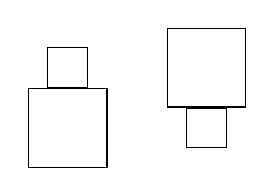
\begin{tikzpicture}
[st/.style={
rectangle,
minimum size=1cm,
node distance=1cm,
inner sep = 0cm,
draw=black,thick,fill=#1!50,
font=\sffamily
},
st/.default=gray]
\node (maj1)[rectangle,draw=black,                     minimum size=.5cm] { };
 \node (min1)[rectangle,draw=black, below= 0cm of maj1, minimum size= 1cm] { };
 \node (maj2)[rectangle,draw=black, right=of maj1,      minimum size= 1cm] { };
 \node (min2)[rectangle,draw=black, below=0cm of maj2,  minimum size=.5cm] { }; 
\end{tikzpicture}
\vspace{12pt}

\caption{Geometric scheme of the major/minor minor/major triads}\label{fig:maj-minor-scheme}
\end{figure}
The thing is that triads are the most used musical structure in music. They offer no doubt, they are like the atoms with which the rest of matter is formed: they are indivisible (there is nothing with a more basic structure) and even when they are not there, the brain ends up finding its footprint. They form the base upon which music rests.
Major triads form a minor/major structure (minor over major) and minor triads form a major/minor structure (major over minor). The subconscious takes these structures as real forms and tries to interpret them.
It is very easy to observe this with any instrument. Listening to a major chord and the same minor chord and asking yourself why the major chord suggests joy and the minor one sadness is the first question we should ask ourselves, and not accept magical'' answers. Over the years, I have heard many answers to this question, the most clumsy being that funeral themes have always been done with minor chords and festive themes with major chords. This is the kind ofanswer'' I am referring to.
It is very clear to me that it is simply a matter of a large structure placed on top of a small one, or vice versa. When I listen to the chord I can see it clearly, and if I look at the figures even more, I can even hear the chords just by looking at them. In the world we live in, a large thing on top of a small one is something\ldots{} unfair, not good, not right, it gives the impression that action is needed, to come to its aid, to solve its problem, to leave things in their natural balance. It is not something necessarily unstable, that is not the problem, but something wrong, something that makes us feel in some way dissatisfied, sad.
It is about two different entities. One is bigger than the other, and the bigger one is on top of the smaller one. Whatever it is: two stones, two boxes, two people, two organizations, two countries\ldots{} it's not fair. The idea of ``being on top of'' in the real world suggests weight, gravity, oppression, endurance, domination, slavery. It is one of the rules of common sense. The normal thing is that small entities are supported by large ones, that they use their power, size, height and balance. Life goes on because the big ones support and support the small ones, the adults the children, the powerful the poor, and not vice versa. Seeing a powerful person on the back of a child is the saddest and most dramatic image one can imagine, the opposite is a beautiful idea of collaboration, friendship, generosity and life.
Those chords are present in 99% of music, and even when they are not present, the listener tries to imagine them, as when there are missing strokes in a picture and our imagination fills in the missing ones based on common sense. When we listen to a major or minor triad, we automatically admit those ideas, and, from them, we try to understand what the music is telling us, as well as orienting ourselves in the map they form.
In short, these are the ideas that automatically suggest those three simple notes:
\begin{table}[htbp]
\centering
\begin{tabular}{ll}
\toprule
\textbf{Minor triad} & \textbf{Major triad} \\
\midrule
Injustice & Justice \\
Sadness & Joy \\
Failure & Triumph \\
Death & Life \\
Oppression & Solidarity \\ 
\bottomrule
\end{tabular}
\caption{Impression produced by the triads}\label{tab:triad-impressions}
\end{table}
\subsection{Orientative triads}
The format of a triad allows us to guess what degree of the scale we are in. In a scale there are some major triads and some minor ones. They are obtained simply by adding to each degree of the scale the next two alternate notes. According to the character of the triad we hear, we can assume what degree of the scale we may be in (as when we see a monument on a map and suddenly we are correctly oriented). As there are several triads of each type, there is still \emph{room for deception}.
\subsection{Tritone}
A \emph{tritone} is formed by two notes 3 tones apart. Between them, there are two minor thirds. It would be something like a \emph{minor / minor} structure. It is not useful for expressing the character of a normal triad, it is ambiguous, since it can be inverted and remains the same. The listener tries to guess that it is going to become a normal triad. That, in music, is called \emph{resolving}.
When we are talking and we want the person listening to us to try to find a solution\ldots{} What do we do? Do we place the problem between question marks and wait for the listener to solve it? Eh?. They are called questions, and we ask them every day.
Well, there are also questions in music. They are unresolved chords, chords that do not form a major or minor structure, and that the listener will not be able to avoid trying to resolve in their head before hearing the next note, chords that require their participation, active listening.
In a scale where two alternate notes are 3 tones apart, the chord that is formed at that degree will sound like a question that needs an answer. It is no coincidence that in the major scale (the one everyone knows, the one formed by the white keys of the piano, \emph{do, re, mi, fa}\ldots) there is a degree where a tritone is formed: degree 7, that of the note \emph{si}. The alternate notes starting from \emph{si} are \emph{re} and \emph{fa}. Between each pair there is a tone and a half, so in total there are 3 tones, that is, two minor thirds one on top of the other. No one will want to end a song with that chord.
No musical performance will ever end (at least if we want the audience to start applauding) with an unresolved chord. The listener expects us to give them a solution. A few thousandths of a second before, they imagine what we are going to give them. If they are right they will feel satisfied, if not they will be surprised. Many questions will be too stimulating for them and they will probably become saturated. No question will make them lose interest.
\subsection{Tritone repulsion}
A tritone sounds repulsive, two minor thirds don't represent anything stacked together.
It tempts the listener to guess what it will resolve to, it makes them participate, it makes them take risks and makes it possible to deceive and surprise them by resolving it unexpectedly.
It invades their tranquility, requiring them to listen actively and take risks. It condemns them to make mistakes without being able to avoid it. It's like the ``\emph{nothing over here\ldots{} nothing over there}\ldots{}'' of the magicians.
In the Middle Ages, that sound was called \emph{Diabolus in musicae}'' and it seems that it represented some kind of challenge to power. The name alone denotes the annoying and even dangerous character it can have, especially if you are a medieval state and use music to keep the masses asleep. Banning the tritone is like when the bad guy in the movie saysI'm the one asking the questions here!''
\subsection{Distance to the tritone}
It is the distance that a degree of the scale maintains with respect to some tritone. If in a scale there is only one tritone, there will be degrees that are far away from it, but if there are two, as we move away from one we get closer to the other, so we will always be close to one of them.
The degrees that are very far away from some tritone suggest stability, relaxation. There are scales that do not contain any tritone. The feeling of linearity and stability (and possibly monotony) is quite strong in them. It is no coincidence that we used them in our primitive stages of civilization. We will delve into this later.
\subsection{Misorientation}
In traditional notation, the degree farthest from the tritone is called \emph{fundamental}, and it is also considered that the scale begins and ends on that degree. This is a serious error; that a degree is far from a tritone does not mean that it is the beginning. This is done because the listener feels comfortable when a song ends on the fundamental degree, as is usually the case. As we have already said, this is one of the serious errors that we want to solve: the angle from which music is seen, the excessive prominence of the listener, (obviously because he is the one who pays and the one who decides whether the composer will succeed or not). In any case, we need to continue composing music for humans, so we will have to continue taking into account what makes them feel comfortable or not, but we need to understand why.
\subsection{Symmetrical Orientation}
The scales we use are symmetrical. Symmetry is a pattern that helps the listener recognize harmony. If a scale is symmetrical, it will help us a lot in its analysis to use a notation that respects this symmetry, where the central point is graphically represented in the center. In the notation we present, this idea is very important.
\subsection{Scales}
These are the scales that are commonly used and the names that have been assigned to them. In standard notation, the equivalence would be as follows:
\begin{table}[htbp]
\centering
\begin{tabular}{lll}
\toprule
\textbf{\textsf{Scale}} & \textbf{Name} & \textbf{Standard} \\
\midrule
\textsf{WHITE} & Diatonic scale & \\
\textsf{BLUE} & Melodic minor scale & \\
\textsf{RED} & Harmonic minor scale & \\
\textsf{BLACK} & Diminished scale & \\
\textsf{PENTA} & Pentatonic scale & \\
\textsf{TONES} & Whole tone scale & \\
\bottomrule
\end{tabular}
\caption{Table of musical scales}\label{tab:scale-name-equivalences}
\end{table}
In the notation created, the degrees of the scale are represented as numbers. It should be noted that the first degree of the scale is not, as in traditional notation, the degree farthest from the tritone (in the diatonic scale it would be DO), but the degree that, as the figures show, occupies the center of the structure (in the diatonic scale it would be RE). Starting from the initial note and rotating clockwise, we go up a tone until we return to the initial tone, that is, we go up an octave.
\begin{figure}[H]
\begin{subfigure}{0.15\textwidth}
\centering
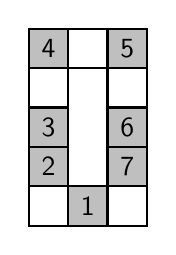
\begin{tikzpicture}
[st/.style={
rectangle,
minimum size=.5cm,
node distance=.5cm,
inner sep = 0cm,
draw=black,thick,fill=#1!50,
font=\sffamily
},
st/.default=gray]
\node (15)[st                   ] {4}; \node (25) [st=white, right of=15] { }; \node (35) [st,       right of= 25] {5};
    \node (14)[st=white,below of= 15] { };                                         \node (34) [st=white, below of= 35] { };
    \node (13)[st,      below of= 14] {3};                                         \node (33) [st,       below of= 34] {6};
    \node (12)[st,      below of= 13] {2};                                         \node (32) [st,       below of= 33] {7};
    \node (11)[st=white,below of= 12] { }; \node (21) [st,       right of=11] {1}; \node (31) [st=white, right of= 21] { };

  \end{tikzpicture}
\caption{\textsf{WHITE}}

\end{subfigure}
\hfill
\begin{subfigure}{0.15\textwidth}
\centering
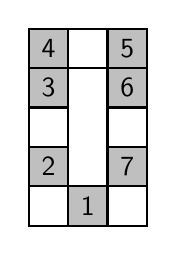
\begin{tikzpicture}
[st/.style={
rectangle,
minimum size=.5cm,
node distance=.5cm,
inner sep = 0cm,
draw=black,thick,fill=#1!50,
font=\sffamily
},
st/.default=gray]
\node (15)[st,                  ] {4}; \node (25) [st=white, right of=15] { }; \node (35) [st,       right of= 25] {5};
    \node (14)[st,      below of= 15] {3};                                         \node (34) [st,       below of= 35] {6};
    \node (13)[st=white,below of= 14] { };                                         \node (33) [st=white, below of= 34] { };
    \node (12)[st,      below of= 13] {2};                                         \node (32) [st,       below of= 33] {7};
    \node (11)[st=white,below of= 12] { }; \node (21) [st,       right of=11] {1}; \node (31) [st=white, right of= 21] { };

  \end{tikzpicture}
\caption{\textsf{BLUE}}

\end{subfigure}
\hfill
\begin{subfigure}{0.15\textwidth}
\centering
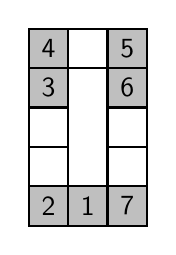
\begin{tikzpicture}
[st/.style={
rectangle,
minimum size=.5cm,
node distance=.5cm,
inner sep = 0cm,
draw=black,thick,fill=#1!50,
font=\sffamily
},
st/.default=gray]
\node (15)[st,                  ] {4}; \node (25) [st=white, right of=15] { }; \node (35) [st,       right of =25] {5};
  \node (14)[st,      below of= 15] {3};                                         \node (34) [st,       below of =35] {6};
  \node (13)[st=white,below of= 14] { };                                         \node (33) [st=white, below of =34] { };
  \node (12)[st=white,below of= 13] { };                                         \node (32) [st=white, below of =33] { };
  \node (11)[st,      below of= 12] {2}; \node (21) [st,       right of=11] {1}; \node (31) [st,       right of =21] {7};

\end{tikzpicture}    
\caption{\textsf{RED}}

\end{subfigure}
\hfill
\begin{subfigure}{0.15\textwidth}
\centering
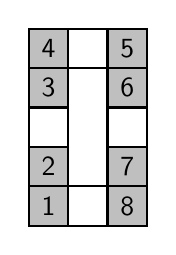
\begin{tikzpicture}
[st/.style={
rectangle,
minimum size=.5cm,
node distance=.5cm,
inner sep = 0cm,
draw=black,thick,fill=#1!50,
font=\sffamily
},
st/.default=gray]
\node (15)[st,                  ] {4}; \node (25) [st=white, right of=15] { }; \node (35) [st,       right of =25] {5};
  \node (14)[st,      below of= 15] {3};                                         \node (34) [st,       below of =35] {6};
  \node (13)[st=white,below of= 14] { };                                         \node (33) [st=white, below of =34] { };
  \node (12)[st      ,below of= 13] {2};                                         \node (32) [st,       below of =33] {7};
  \node (11)[st,      below of= 12] {1}; \node (21) [st=white, right of=11] { }; \node (31) [st,       right of =21] {8};

\end{tikzpicture}   
\caption{\textsf{BLACK}}

\end{subfigure}
\hfill
\begin{subfigure}{0.15\textwidth}
\centering
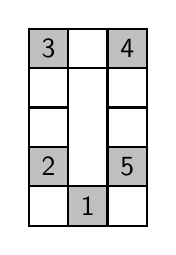
\begin{tikzpicture}
[st/.style={
rectangle,
minimum size=.5cm,
node distance=.5cm,
inner sep = 0cm,
draw=black,thick,fill=#1!50,
font=\sffamily
},
st/.default=gray]
\node (15)[st                   ] {3}; \node (25) [st=white, right of=15] { }; \node (35) [st,       right of= 25] {4};
  \node (14)[st=white,below of= 15] { };                                         \node (34) [st=white, below of= 35] { };
  \node (13)[st=white,below of= 14] { };                                         \node (33) [st=white, below of= 34] { };
  \node (12)[st,      below of= 13] {2};                                         \node (32) [st,       below of= 33] {5};
\node (11)[st=white,below of= 12] { }; \node (21) [st, right of=11] {1}; \node (31) [st=white, right of= 21] { };
\end{tikzpicture}    
\caption{\textsf{PENTA}}

\end{subfigure}
\hfill
\begin{subfigure}{0.15\textwidth}
\centering
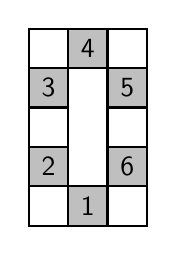
\begin{tikzpicture}
[st/.style={
rectangle,
minimum size=.5cm,
node distance=.5cm,
inner sep = 0cm,
draw=black,thick,fill=#1!50,
font=\sffamily
},
st/.default=gray]
\node (15)[st=white             ] { }; \node (25) [st,       right of=15] {4}; \node (35) [st=white, right of= 25] { };
  \node (14)[st,      below of= 15] {3};                                         \node (34) [st,       below of= 35] {5};
  \node (13)[st=white,below of= 14] { };                                         \node (33) [st=white, below of= 34] { };
  \node (12)[st,      below of= 13] {2};                                         \node (32) [st,       below of= 33] {6};
  \node (11)[st=white,below of= 12] { }; \node (21) [st,       right of=11] {1}; \node (31) [st=white, right of= 21] { };

\end{tikzpicture}   
\caption{\textsf{TONES}}

\end{subfigure}
\hfill
\caption{The six scales}\label{fig:the-six-scales}
\end{figure}
Note that in the \textsf{BLACK} scale, the symmetry is not based on the notes, but on the space between them, and there is not a central note, but a space between notes in the center. The feeling of symmetry that the listener perceives is identical and the notation reflects this.
This notation is very simple, portable and practical. At a glance, one can observe the symmetry of all the scales. If you compare it with traditional notation, where no symmetry is appreciated, you will notice an incredible improvement in the possibilities it offers for analysis, study and assimilation.
\subsection{Names of the scales}
Following the same line of reasoning, we will stop referring to a scale with the name of the note that is farthest from the tritone, and we will use its central note. For example, the scale that has no sharps will no longer be called C scale'', and will becomeD scale''. The note that names a scale is its central note, not the note that seems to us to suggest rest, fullness or resolution.
A particular case would be that of the \textsf{BLACK} scale. As we have seen, the central note is not such a thing, but a space between two notes. So when referring to the \textsf{BLACK} scale of F we are indicating the scale whose first note after the space is an F.
\subsection{Names of the notes}
We will represent the notes of the scale using American notation, that is, using the letters from A to G, but with a slight modification: there are no \emph{sharps}.
\begin{table}[htbp]
\centering
\begingroup
\sffamily
\begin{tabular}{*{12}{c}}
\toprule
A & A$\sharp$ B$\flat$ & B & C & C$\sharp$ D$\flat$ & D & D$\sharp$ E$\flat$ & E & F & F$\sharp$ G$\flat$ & G & G$\sharp$ A$\flat$ \\
\midrule
A & b & B & C & d & D & e & E & F & g & G & a \\
\bottomrule
\end{tabular}
\endgroup
\caption{Equivalences of the notes}\label{tab:note-equivalences}
\end{table}
In standard notation, when you want to raise a note a semitone you put the sharp sign ($\sharp$) and when you want to lower it a semitone, you add a flat ($\flat$), so C$\sharp$ is actually the same note as D$\flat$.
In our notation, to indicate flats we use the same letter but in lowercase. So in the same scale you can find a natural note and also the same flat note. For example, the note \texttt{b} is equivalent to both \texttt{A$\sharp$} and \texttt{B$\flat$}:
This would be the representation of the \texttt{BLUE} scale of \texttt{A}, that is, of \texttt{A}. We observe that the \texttt{D flat\ (d)} appears and then the \texttt{D natural\ (D)}.
\begin{figure}[h]
\centering
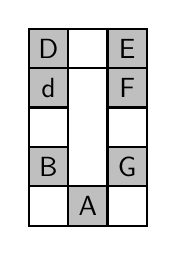
\begin{tikzpicture}
[st/.style={
rectangle,
minimum size=.5cm,
node distance=.5cm,
inner sep = 0cm,
draw=black,thick,fill=#1!50,
font=\sffamily
},
st/.default=gray]
\node (15)[st                     ] {D}; \node (25) [st=white, right of= 15] { }; \node (35) [st, right of=25       ] {E};
\node (14)[st,       below of= 15 ] {d};                                          \node (34) [st,       below of =35] {F};
\node (13)[st=white, below of = 14] { };                                          \node (33) [st=white, below of =34] { };
\node (12)[st,       below of = 13] {B};                                          \node (32) [st, below of= 33      ] {G};
\node (11)[st=white, below of= 12 ] { }; \node (21) [right of=11, st      ] {A};  \node (31) [right of= 21, st=white] { };

\end{tikzpicture}
\vspace{12pt}
\caption{The BLUE scale of A}\label{fig:blue-scale-of-a}
\end{figure}
\subsection{Modes}
Modes are the different ``views'' of existing scales, that is, the same scale taken starting from different notes.
From the scales presented, these modes are generated. For now, we have assigned a number to each (let's not invent names, if possible!), taking zero as the central mode and then positive or negative numbers if we go down or up the scale.
The historical names of the modes are directly taken from Greek culture, they are \textsf{Dorian}, \textsf{Ionian}, \textsf{Mixolydian}\ldots etc. As if they were ancient buildings. And let's not talk about the modes of the melodic minor scale (our \textsf{BLUE} scale), \textsf{Phrygian augmented}, \textsf{Lydian$\sharp$4}, \textsf{Locrian$\sharp$2}, \textsf{Superlocrian $\flat$$\flat$7}. No doubt something needs to be done to stop using these outlandish ``proto-phonetic'' artifacts of antiquity.
\begin{figure}[H]
\begin{subfigure}{0.10\textwidth}
\centering
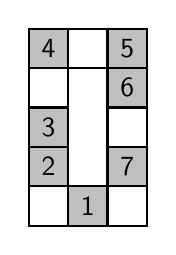
\begin{tikzpicture}
[st/.style={
rectangle,
minimum size=.5cm,
node distance=.5cm,
inner sep = 0cm,
draw=black,thick,fill=#1!50,
font=\sffamily
},
st/.default=gray]
\node (15)[st                   ] {4}; \node (25) [st=white, right of=15] { }; \node (35) [st,       right of= 25] {5};
  \node (14)[st=white,below of= 15] { };                                         \node (34) [st,       below of= 35] {6};
  \node (13)[st,      below of= 14] {3};                                         \node (33) [st=white, below of= 34] { };
  \node (12)[st,      below of= 13] {2};                                         \node (32) [st,       below of= 33] {7};
  \node (11)[st=white,below of= 12] { }; \node (21) [st,       right of=11] {1}; \node (31) [st=white, right of= 21] { };

\end{tikzpicture}    
\caption{\textsf{-3}}

\end{subfigure}
\hfill
\begin{subfigure}{0.10\textwidth}
\centering
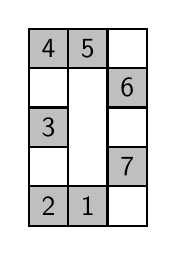
\begin{tikzpicture}
[st/.style={
rectangle,
minimum size=.5cm,
node distance=.5cm,
inner sep = 0cm,
draw=black,thick,fill=#1!50,
font=\sffamily
},
st/.default=gray]
\node (15)[st                   ] {4}; \node (25) [st,       right of=15] {5}; \node (35) [st=white, right of= 25] { };
  \node (14)[st=white,below of= 15] { };                                         \node (34) [st,       below of= 35] {6};
  \node (13)[st,      below of= 14] {3};                                         \node (33) [st=white, below of= 34] { };
  \node (12)[st=white,below of= 13] { };                                         \node (32) [st,       below of= 33] {7};
  \node (11)[st,      below of= 12] {2}; \node (21) [st,       right of=11] {1}; \node (31) [st=white, right of= 21] { };

\end{tikzpicture}    
\caption{\textsf{-2}}

\end{subfigure}
\hfill
\begin{subfigure}{0.10\textwidth}
\centering
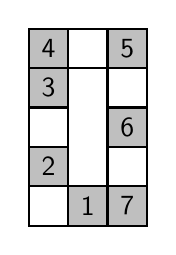
\begin{tikzpicture}
[st/.style={
rectangle,
minimum size=.5cm,
node distance=.5cm,
inner sep = 0cm,
draw=black,thick,fill=#1!50,
font=\sffamily
},
st/.default=gray]
\node (15)[st                   ] {4}; \node (25) [st=white, right of=15] { }; \node (35) [st,       right of= 25] {5};
  \node (14)[st,      below of= 15] {3};                                         \node (34) [st=white, below of= 35] { };
  \node (13)[st=white,below of= 14] { };                                         \node (33) [st,       below of= 34] {6};
  \node (12)[st,      below of= 13] {2};                                         \node (32) [st=white, below of= 33] { };
  \node (11)[st=white,below of= 12] { }; \node (21) [st,       right of=11] {1}; \node (31) [st,       right of= 21] {7};

\end{tikzpicture}    
\caption{\textsf{-1}}

\end{subfigure}
\hfill
\begin{subfigure}{0.10\textwidth}
\centering
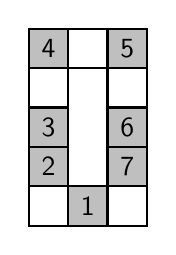
\begin{tikzpicture}
[st/.style={
rectangle,
minimum size=.5cm,
node distance=.5cm,
inner sep = 0cm,
draw=black,thick,fill=#1!50,
font=\sffamily
},
st/.default=gray]
\node (15)[st                   ] {4}; \node (25) [st=white, right of=15] { }; \node (35) [st,       right of= 25] {5};
    \node (14)[st=white,below of= 15] { };                                         \node (34) [st=white, below of= 35] { };
    \node (13)[st,      below of= 14] {3};                                         \node (33) [st,       below of= 34] {6};
    \node (12)[st,      below of= 13] {2};                                         \node (32) [st,       below of= 33] {7};
    \node (11)[st=white,below of= 12] { }; \node (21) [st,       right of=11] {1}; \node (31) [st=white, right of= 21] { };

  \end{tikzpicture}
\caption{\textsf{0}}

\end{subfigure}
\hfill
\begin{subfigure}{0.10\textwidth}
\centering
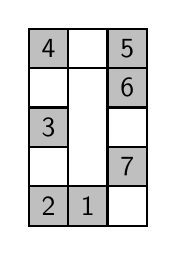
\begin{tikzpicture}
[st/.style={
rectangle,
minimum size=.5cm,
node distance=.5cm,
inner sep = 0cm,
draw=black,thick,fill=#1!50,
font=\sffamily
},
st/.default=gray]
\node (15)[st,                  ] {4}; \node (25) [st=white, right of=15] { }; \node (35) [st,       right of= 25] {5};
    \node (14)[st=white,below of= 15] { };                                         \node (34) [st,       below of= 35] {6};
    \node (13)[st,      below of= 14] {3};                                         \node (33) [st=white, below of= 34] { };
    \node (12)[st=white,below of= 13] { };                                         \node (32) [st,       below of= 33] {7};
    \node (11)[st      ,below of= 12] {2}; \node (21) [st,       right of=11] {1}; \node (31) [st=white, right of= 21] { };

  \end{tikzpicture}
\caption{\textsf{+1}}

\end{subfigure}
\hfill
\begin{subfigure}{0.10\textwidth}
\centering
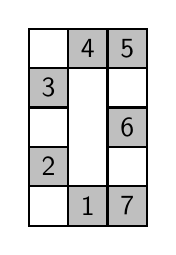
\begin{tikzpicture}
[st/.style={
rectangle,
minimum size=.5cm,
node distance=.5cm,
inner sep = 0cm,
draw=black,thick,fill=#1!50,
font=\sffamily
},
st/.default=gray]
\node (15)[st=white,            ] { }; \node (25) [st,       right of=15] {4}; \node (35) [st,       right of =25] {5};
  \node (14)[st,      below of= 15] {3};                                         \node (34) [st=white, below of =35] { };
  \node (13)[st=white,below of= 14] { };                                         \node (33) [st,       below of =34] {6};
  \node (12)[st,      below of= 13] {2};                                         \node (32) [st=white, below of =33] { };
  \node (11)[st=white,below of= 12] { }; \node (21) [st,       right of=11] {1}; \node (31) [st,       right of =21] {7};

\end{tikzpicture}    
\caption{\textsf{+2}}

\end{subfigure}
\hfill
\begin{subfigure}{0.10\textwidth}
\centering
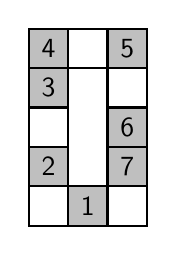
\begin{tikzpicture}
[st/.style={
rectangle,
minimum size=.5cm,
node distance=.5cm,
inner sep = 0cm,
draw=black,thick,fill=#1!50,
font=\sffamily
},
st/.default=gray]
\node (15)[st,                  ] {4}; \node (25) [st=white, right of=15] { }; \node (35) [st,       right of =25] {5};
  \node (14)[st,      below of= 15] {3};                                         \node (34) [st=white, below of =35] { };
  \node (13)[st=white,below of= 14] { };                                         \node (33) [st,       below of =34] {6};
  \node (12)[st      ,below of= 13] {2};                                         \node (32) [st,       below of =33] {7};
  \node (11)[st=white,below of= 12] { }; \node (21) [st,       right of=11] {1}; \node (31) [st=white, right of =21] { };

\end{tikzpicture}    
\caption{\textsf{+3}}

\end{subfigure}
\hfill
\caption{The seven modes of \textsf{WHITE}}\label{fig:the-white-modes}
\end{figure}
\begin{figure}[H]
\begin{subfigure}{0.10\textwidth}
\centering
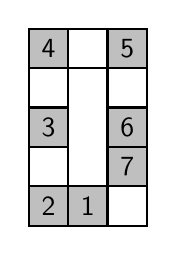
\begin{tikzpicture}
[st/.style={
rectangle,
minimum size=.5cm,
node distance=.5cm,
inner sep = 0cm,
draw=black,thick,fill=#1!50,
font=\sffamily
},
st/.default=gray]
\node (15)[st                   ] {4}; \node (25) [st=white, right of=15] { }; \node (35) [st,       right of= 25] {5};
  \node (14)[st=white,below of= 15] { };                                         \node (34) [st=white, below of= 35] { };
  \node (13)[st,      below of= 14] {3};                                         \node (33) [st,       below of= 34] {6};
  \node (12)[st=white,below of= 13] { };                                         \node (32) [st,       below of= 33] {7};
  \node (11)[st,      below of= 12] {2}; \node (21) [st,       right of=11] {1}; \node (31) [st=white, right of= 21] { };

\end{tikzpicture}    
\caption{\textsf{-3}}

\end{subfigure}
\hfill
\begin{subfigure}{0.10\textwidth}
\centering
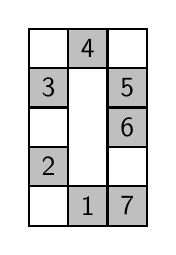
\begin{tikzpicture}
[st/.style={
rectangle,
minimum size=.5cm,
node distance=.5cm,
inner sep = 0cm,
draw=black,thick,fill=#1!50,
font=\sffamily
},
st/.default=gray]
\node (15)[st=white             ] { }; \node (25) [st,       right of=15] {4}; \node (35) [st=white, right of= 25] { };
  \node (14)[st,      below of= 15] {3};                                         \node (34) [st,       below of= 35] {5};
  \node (13)[st=white,below of= 14] { };                                         \node (33) [st,       below of= 34] {6};
  \node (12)[st,      below of= 13] {2};                                         \node (32) [st=white, below of= 33] { };
  \node (11)[st=white,below of= 12] { }; \node (21) [st,       right of=11] {1}; \node (31) [st,       right of= 21] {7};

\end{tikzpicture}    
\caption{\textsf{-2}}

\end{subfigure}
\hfill
\begin{subfigure}{0.10\textwidth}
\centering
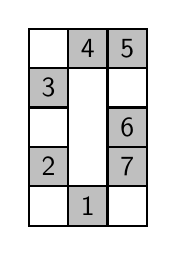
\begin{tikzpicture}
[st/.style={
rectangle,
minimum size=.5cm,
node distance=.5cm,
inner sep = 0cm,
draw=black,thick,fill=#1!50,
font=\sffamily
},
st/.default=gray]
\node (15)[st=white             ] { }; \node (25) [st,       right of=15] {4}; \node (35) [st,       right of= 25] {5};
  \node (14)[st,      below of= 15] {3};                                         \node (34) [st=white, below of= 35] { };
  \node (13)[st=white,below of= 14] { };                                         \node (33) [st,       below of= 34] {6};
  \node (12)[st,      below of= 13] {2};                                         \node (32) [st,       below of= 33] {7};
  \node (11)[st=white,below of= 12] { }; \node (21) [st,       right of=11] {1}; \node (31) [st=white, right of= 21] { };

\end{tikzpicture}    
\caption{\textsf{-1}}

\end{subfigure}
\hfill
\begin{subfigure}{0.10\textwidth}
\centering
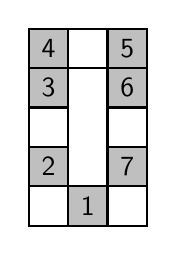
\begin{tikzpicture}
[st/.style={
rectangle,
minimum size=.5cm,
node distance=.5cm,
inner sep = 0cm,
draw=black,thick,fill=#1!50,
font=\sffamily
},
st/.default=gray]
\node (15)[st                   ] {4}; \node (25) [st=white, right of=15] { }; \node (35) [st,       right of= 25] {5};
    \node (14)[st,      below of= 15] {3};                                         \node (34) [st,       below of= 35] {6};
    \node (13)[st=white,below of= 14] { };                                         \node (33) [st=white, below of= 34] { };
    \node (12)[st,      below of= 13] {2};                                         \node (32) [st,       below of= 33] {7};
    \node (11)[st=white,below of= 12] { }; \node (21) [st,       right of=11] {1}; \node (31) [st=white, right of= 21] { };

  \end{tikzpicture}
\caption{\textsf{0}}

\end{subfigure}
\hfill
\begin{subfigure}{0.10\textwidth}
\centering
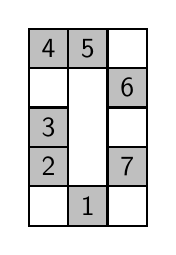
\begin{tikzpicture}
[st/.style={
rectangle,
minimum size=.5cm,
node distance=.5cm,
inner sep = 0cm,
draw=black,thick,fill=#1!50,
font=\sffamily
},
st/.default=gray]
\node (15)[st,                  ] {4}; \node (25) [st,       right of=15] {5}; \node (35) [st=white, right of= 25] { };
    \node (14)[st=white,below of= 15] { };                                         \node (34) [st,       below of= 35] {6};
    \node (13)[st,      below of= 14] {3};                                         \node (33) [st=white, below of= 34] { };
    \node (12)[st,      below of= 13] {2};                                         \node (32) [st,       below of= 33] {7};
    \node (11)[st=white,below of= 12] { }; \node (21) [st,       right of=11] {1}; \node (31) [st=white, right of= 21] { };

  \end{tikzpicture}
\caption{\textsf{+1}}

\end{subfigure}
\hfill
\begin{subfigure}{0.10\textwidth}
\centering
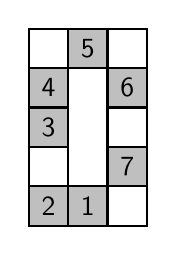
\begin{tikzpicture}
[st/.style={
rectangle,
minimum size=.5cm,
node distance=.5cm,
inner sep = 0cm,
draw=black,thick,fill=#1!50,
font=\sffamily
},
st/.default=gray]
\node (15)[st=white,            ] { }; \node (25) [st,       right of=15] {5}; \node (35) [st=white, right of =25] { };
  \node (14)[st,      below of= 15] {4};                                         \node (34) [st,       below of =35] {6};
  \node (13)[st,      below of= 14] {3};                                         \node (33) [st=white, below of =34] { };
  \node (12)[st=white,below of= 13] { };                                         \node (32) [st,       below of =33] {7};
  \node (11)[st,      below of= 12] {2}; \node (21) [st,       right of=11] {1}; \node (31) [st=white, right of =21] { };

\end{tikzpicture}    
\caption{\textsf{+2}}

\end{subfigure}
\hfill
\begin{subfigure}{0.10\textwidth}
\centering
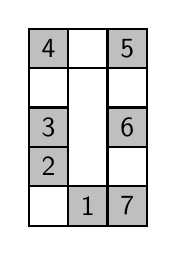
\begin{tikzpicture}
[st/.style={
rectangle,
minimum size=.5cm,
node distance=.5cm,
inner sep = 0cm,
draw=black,thick,fill=#1!50,
font=\sffamily
},
st/.default=gray]
\node (15)[st,                  ] {4}; \node (25) [st=white, right of=15] { }; \node (35) [st,       right of =25] {5};
  \node (14)[st=white,below of= 15] { };                                         \node (34) [st=white, below of =35] { };
  \node (13)[st,      below of= 14] {3};                                         \node (33) [st,       below of =34] {6};
  \node (12)[st      ,below of= 13] {2};                                         \node (32) [st=white, below of =33] { };
  \node (11)[st=white,below of= 12] { }; \node (21) [st,       right of=11] {1}; \node (31) [st,       right of =21] {7};

\end{tikzpicture}    
\caption{\textsf{+3}}

\end{subfigure}
\hfill
\caption{The seven modes of \textsf{BLUE}}\label{fig:the-blue-modes}
\end{figure}
\begin{figure}[H]
\begin{subfigure}{0.10\textwidth}
\centering
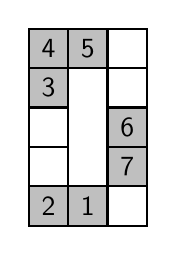
\begin{tikzpicture}
[st/.style={
rectangle,
minimum size=.5cm,
node distance=.5cm,
inner sep = 0cm,
draw=black,thick,fill=#1!50,
font=\sffamily
},
st/.default=gray]
\node (15)[st                   ] {4}; \node (25) [st,       right of=15] {5}; \node (35) [st=white, right of= 25] { };
    \node (14)[st,      below of= 15] {3};                                         \node (34) [st=white, below of= 35] { };
    \node (13)[st=white,below of= 14] { };                                         \node (33) [st,       below of= 34] {6};
    \node (12)[st=white,below of= 13] { };                                         \node (32) [st,       below of= 33] {7};
    \node (11)[st,      below of= 12] {2}; \node (21) [st,       right of=11] {1}; \node (31) [st=white, right of= 21] { };
  
  \end{tikzpicture}    
  \caption{\textsf{-3}}
  
\end{subfigure}
\hfill
\begin{subfigure}{0.10\textwidth}
  \centering
  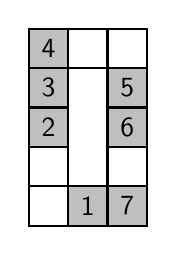
\begin{tikzpicture}
    [st/.style={
      rectangle,
      minimum size=.5cm,
      node distance=.5cm,
      inner sep = 0cm,      
      draw=black,thick,fill=#1!50,
      font=\sffamily
      },
    st/.default=gray]    

    \node (15)[st                   ] {4}; \node (25) [st=white, right of=15] { }; \node (35) [st=white, right of= 25] { };
    \node (14)[st,      below of= 15] {3};                                         \node (34) [st,       below of= 35] {5};
    \node (13)[st,      below of= 14] {2};                                         \node (33) [st,       below of= 34] {6};
    \node (12)[st=white,below of= 13] { };                                         \node (32) [st=white, below of= 33] { };
    \node (11)[st=white,below of= 12] { }; \node (21) [st,       right of=11] {1}; \node (31) [st,       right of= 21] {7};
  
  \end{tikzpicture}    
  \caption{\textsf{-2}}
  
\end{subfigure}
\hfill
\begin{subfigure}{0.10\textwidth}
  \centering
  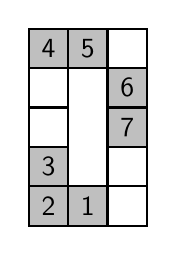
\begin{tikzpicture}
    [st/.style={
      rectangle,
      minimum size=.5cm,
      node distance=.5cm,
      inner sep = 0cm,      
      draw=black,thick,fill=#1!50,
      font=\sffamily
      },
    st/.default=gray] 

    \node (15)[st                   ] {4}; \node (25) [st,       right of=15] {5}; \node (35) [st=white, right of= 25] { };
    \node (14)[st=white,below of= 15] { };                                         \node (34) [st,       below of= 35] {6};
    \node (13)[st=white,below of= 14] { };                                         \node (33) [st,       below of= 34] {7};
    \node (12)[st,      below of= 13] {3};                                         \node (32) [st=white, below of= 33] { };
    \node (11)[st,      below of= 12] {2}; \node (21) [st,       right of=11] {1}; \node (31) [st=white, right of= 21] { };

  \end{tikzpicture}    
  \caption{\textsf{-1}}
  
\end{subfigure}
\hfill
\begin{subfigure}{0.10\textwidth}
  \centering
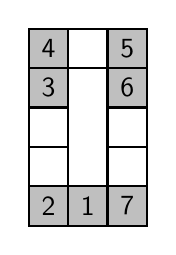
\begin{tikzpicture}
[st/.style={
rectangle,
minimum size=.5cm,
node distance=.5cm,
inner sep = 0cm,
draw=black,thick,fill=#1!50,
font=\sffamily
},
st/.default=gray]
\node (15)[st                   ] {4}; \node (25) [st=white, right of=15] { }; \node (35) [st,       right of= 25] {5};
      \node (14)[st,      below of= 15] {3};                                         \node (34) [st,       below of= 35] {6};
      \node (13)[st=white,below of= 14] { };                                         \node (33) [st=white, below of= 34] { };
      \node (12)[st=white,below of= 13] { };                                         \node (32) [st=white, below of= 33] { };
      \node (11)[st,      below of= 12] {2}; \node (21) [st,       right of=11] {1}; \node (31) [st,       right of= 21] {7};
  
    \end{tikzpicture}
  \caption{\textsf{0}}
  
\end{subfigure}
\hfill
\begin{subfigure}{0.10\textwidth}
  \centering
    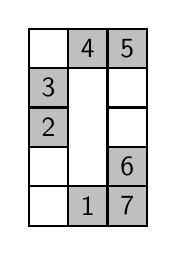
\begin{tikzpicture}
      [st/.style={
        rectangle,
        minimum size=.5cm,
        node distance=.5cm,
        inner sep = 0cm,      
        draw=black,thick,fill=#1!50,
        font=\sffamily
        },
      st/.default=gray]
  
      \node (15)[st=white,            ] { }; \node (25) [st,       right of=15] {4}; \node (35) [st,       right of= 25] {5};
      \node (14)[st,      below of= 15] {3};                                         \node (34) [st=white, below of= 35] { };
      \node (13)[st,      below of= 14] {2};                                         \node (33) [st=white, below of= 34] { };
      \node (12)[st=white,below of= 13] { };                                         \node (32) [st,       below of= 33] {6};
      \node (11)[st=white,below of= 12] { }; \node (21) [st,       right of=11] {1}; \node (31) [st,       right of= 21] {7};
  
    \end{tikzpicture}
  \caption{\textsf{+1}}
  
\end{subfigure}
\hfill
\begin{subfigure}{0.10\textwidth}
  \centering
    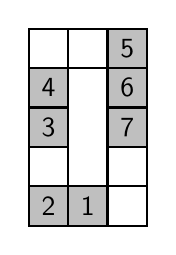
\begin{tikzpicture}
      [st/.style={
        rectangle,
        minimum size=.5cm,
        node distance=.5cm,
        inner sep = 0cm,      
        draw=black,thick,fill=#1!50,
        font=\sffamily
        },
      st/.default=gray]
  
      \node (15)[st=white,            ] { }; \node (25) [st=white, right of=15] { }; \node (35) [st,       right of =25] {5};
      \node (14)[st,      below of= 15] {4};                                         \node (34) [st,       below of =35] {6};
      \node (13)[st,      below of= 14] {3};                                         \node (33) [st,       below of =34] {7};
      \node (12)[st=white,below of= 13] { };                                         \node (32) [st=white, below of =33] { };
      \node (11)[st,      below of= 12] {2}; \node (21) [st,       right of=11] {1}; \node (31) [st=white, right of =21] { };

  \end{tikzpicture}    
  \caption{\textsf{+2}}
  
\end{subfigure}
\hfill
\begin{subfigure}{0.10\textwidth}
  \centering
  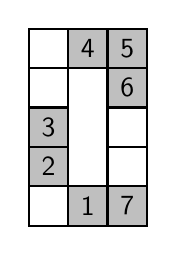
\begin{tikzpicture}
    [st/.style={
      rectangle,
      minimum size=.5cm,
      node distance=.5cm,
      inner sep = 0cm,      
      draw=black,thick,fill=#1!50,
      font=\sffamily
      },
    st/.default=gray]

    \node (15)[st=white,            ] { }; \node (25) [st,       right of=15] {4}; \node (35) [st,       right of =25] {5};
    \node (14)[st=white,below of= 15] { };                                         \node (34) [st,       below of =35] {6};
    \node (13)[st,      below of= 14] {3};                                         \node (33) [st=white, below of =34] { };
    \node (12)[st      ,below of= 13] {2};                                         \node (32) [st=white, below of =33] { };
    \node (11)[st=white,below of= 12] { }; \node (21) [st,       right of=11] {1}; \node (31) [st,       right of =21] {7};

  \end{tikzpicture}    
  \caption{\textsf{+3}}
  
\end{subfigure}
\hfill
\caption{The seven modes of \textsf{RED}}\label{fig:the-red-modes}

\end{figure}
\begin{figure}[H]
\begin{subfigure}{0.10\textwidth}
\centering
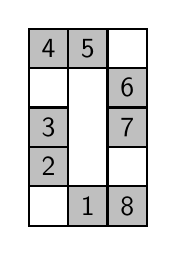
\begin{tikzpicture}
[st/.style={
rectangle,
minimum size=.5cm,
node distance=.5cm,
inner sep = 0cm,
draw=black,thick,fill=#1!50,
font=\sffamily
},
st/.default=gray]
\node (15)[st                   ] {4}; \node (25) [st,       right of=15] {5}; \node (35) [st=white, right of= 25] { };
    \node (14)[st=white,below of= 15] { };                                         \node (34) [st,       below of= 35] {6};
    \node (13)[st,      below of= 14] {3};                                         \node (33) [st,       below of= 34] {7};
    \node (12)[st,      below of= 13] {2};                                         \node (32) [st=white, below of= 33] { };
    \node (11)[st=white,below of= 12] { }; \node (21) [st,       right of=11] {1}; \node (31) [st,       right of= 21] {8};

  \end{tikzpicture}    
  \caption{\textsf{-1}}
  
\end{subfigure}  
\hfill    
\begin{subfigure}{0.10\textwidth}
  \centering
    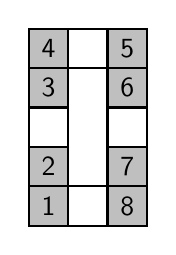
\begin{tikzpicture}
      [st/.style={
        rectangle,
        minimum size=.5cm,
        node distance=.5cm,
        inner sep = 0cm,      
        draw=black,thick,fill=#1!50,
        font=\sffamily
        },
      st/.default=gray]
  
      \node (15)[st                   ] {4}; \node (25) [st=white, right of=15] { }; \node (35) [st,       right of= 25] {5};
      \node (14)[st,      below of= 15] {3};                                         \node (34) [st,       below of= 35] {6};
      \node (13)[st=white,below of= 14] { };                                         \node (33) [st=white, below of= 34] { };
      \node (12)[st,      below of= 13] {2};                                         \node (32) [st,       below of= 33] {7};
      \node (11)[st,      below of= 12] {1}; \node (21) [st=white, right of=11] { }; \node (31) [st,       right of= 21] {8};
  
    \end{tikzpicture}
  \caption{\textsf{0}}
  
\end{subfigure}    
\hfill    
\begin{subfigure}{0.10\textwidth}
  \centering
    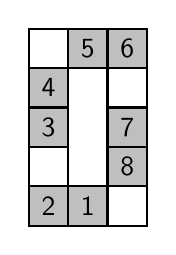
\begin{tikzpicture}
      [st/.style={
        rectangle,
        minimum size=.5cm,
        node distance=.5cm,
        inner sep = 0cm,      
        draw=black,thick,fill=#1!50,
        font=\sffamily
        },
      st/.default=gray]
  
      \node (15)[st=white,            ] { }; \node (25) [st,       right of=15] {5}; \node (35) [st,       right of= 25] {6};
      \node (14)[st,      below of= 15] {4};                                         \node (34) [st=white, below of= 35] { };
      \node (13)[st,      below of= 14] {3};                                         \node (33) [st,       below of= 34] {7};
      \node (12)[st=white,below of= 13] { };                                         \node (32) [st,       below of= 33] {8};
      \node (11)[st,      below of= 12] {2}; \node (21) [st,       right of=11] {1}; \node (31) [st=white, right of= 21] { };
  
    \end{tikzpicture}
  \caption{\textsf{+1}}
  
\end{subfigure}
\hfill
\caption{The three modes of \textsf{BLACK}}\label{fig:the-black-modes}

\end{figure}
\begin{figure}[H]
\begin{subfigure}{0.10\textwidth}
\centering
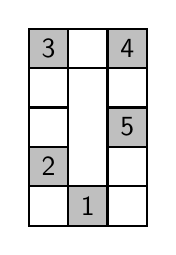
\begin{tikzpicture}
[st/.style={
rectangle,
minimum size=.5cm,
node distance=.5cm,
inner sep = 0cm,
draw=black,thick,fill=#1!50,
font=\sffamily
},
st/.default=gray]
\node (15)[st                   ] {3}; \node (25) [st=white, right of=15] { }; \node (35) [st,       right of= 25] {4};
      \node (14)[st=white,below of= 15] { };                                         \node (34) [st=white, below of= 35] { };
      \node (13)[st=white,below of= 14] { };                                         \node (33) [st,       below of= 34] {5};
      \node (12)[st,      below of= 13] {2};                                         \node (32) [st=white, below of= 33] { };
      \node (11)[st=white,below of= 12] { }; \node (21) [st,       right of=11] {1}; \node (31) [st=white, right of= 21] { };

    \end{tikzpicture}    
    \caption{\textsf{-2}}
    
  \end{subfigure}
  \hfill  
\begin{subfigure}{0.10\textwidth}
  \centering
  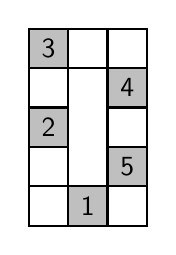
\begin{tikzpicture}
    [st/.style={
      rectangle,
      minimum size=.5cm,
      node distance=.5cm,
      inner sep = 0cm,      
      draw=black,thick,fill=#1!50,
      font=\sffamily
      },
    st/.default=gray] 

    \node (15)[st                   ] {3}; \node (25) [st=white, right of=15] { }; \node (35) [st=white, right of= 25] { };
    \node (14)[st=white,below of= 15] { };                                         \node (34) [st,       below of= 35] {4};
    \node (13)[st,      below of= 14] {2};                                         \node (33) [st=white, below of= 34] { };
    \node (12)[st=white,below of= 13] { };                                         \node (32) [st,       below of= 33] {5};
    \node (11)[st=white,below of= 12] { }; \node (21) [st,       right of=11] {1}; \node (31) [st=white, right of= 21] { };

  \end{tikzpicture}    
  \caption{\textsf{-1}}
  
\end{subfigure}
\hfill
\begin{subfigure}{0.10\textwidth}
  \centering
    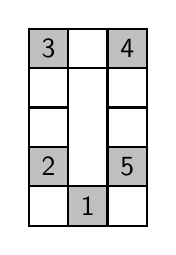
\begin{tikzpicture}
      [st/.style={
        rectangle,
        minimum size=.5cm,
        node distance=.5cm,
        inner sep = 0cm,      
        draw=black,thick,fill=#1!50,
        font=\sffamily
        },
      st/.default=gray]
  
      \node (15)[st                   ] {3}; \node (25) [st=white, right of=15] { }; \node (35) [st,       right of= 25] {4};
      \node (14)[st=white,below of= 15] { };                                         \node (34) [st=white, below of= 35] { };
      \node (13)[st=white,below of= 14] { };                                         \node (33) [st=white, below of= 34] { };
      \node (12)[st,      below of= 13] {2};                                         \node (32) [st,       below of= 33] {5};
      \node (11)[st=white,below of= 12] { }; \node (21) [st,       right of=11] {1}; \node (31) [st=white, right of= 21] { };
  
    \end{tikzpicture}
  \caption{\textsf{0}}
  
\end{subfigure}
\hfill
\begin{subfigure}{0.10\textwidth}
  \centering
    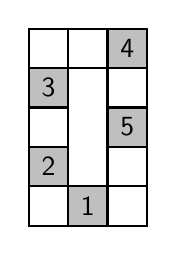
\begin{tikzpicture}
      [st/.style={
        rectangle,
        minimum size=.5cm,
        node distance=.5cm,
        inner sep = 0cm,      
        draw=black,thick,fill=#1!50,
        font=\sffamily
        },
      st/.default=gray]
  
      \node (15)[st=white,            ] { }; \node (25) [st=white, right of=15] { }; \node (35) [st,       right of= 25] {4};
      \node (14)[st,      below of= 15] {3};                                         \node (34) [st=white, below of= 35] { };
      \node (13)[st=white,below of= 14] { };                                         \node (33) [st,       below of= 34] {5};
      \node (12)[st,      below of= 13] {2};                                         \node (32) [st=white, below of= 33] { };
      \node (11)[st=white,below of= 12] { }; \node (21) [st,       right of=11] {1}; \node (31) [st=white, right of= 21] { };
  
    \end{tikzpicture}
  \caption{\textsf{+1}}
  
\end{subfigure}
\hfill
\begin{subfigure}{0.10\textwidth}
  \centering
    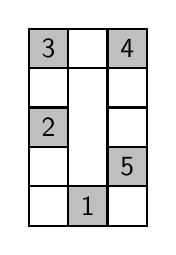
\begin{tikzpicture}
      [st/.style={
        rectangle,
        minimum size=.5cm,
        node distance=.5cm,
        inner sep = 0cm,      
        draw=black,thick,fill=#1!50,
        font=\sffamily
        },
      st/.default=gray]
  
      \node (15)[st,                  ] {3}; \node (25) [st=white, right of=15] { }; \node (35) [st,       right of= 25] {4};
      \node (14)[st=white,below of= 15] { };                                         \node (34) [st=white, below of= 35] { };
      \node (13)[st,      below of= 14] {2};                                         \node (33) [st=white, below of= 34] { };
      \node (12)[st=white,below of= 13] { };                                         \node (32) [st,       below of= 33] {5};
      \node (11)[st=white,below of= 12] { }; \node (21) [st,       right of=11] {1}; \node (31) [st=white, right of= 21] { };
  
    \end{tikzpicture}
  \caption{\textsf{+2}}
  
\end{subfigure}
\caption{The five modes of \textsf{PENTA}}\label{fig:the-penta-modes}

\end{figure}
\begin{figure}[H]
\begin{subfigure}{1\textwidth}
\centering
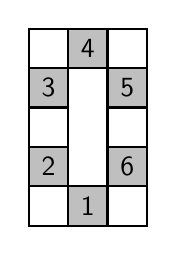
\begin{tikzpicture}
[st/.style={
rectangle,
minimum size=.5cm,
node distance=.5cm,
inner sep = 0cm,
draw=black,thick,fill=#1!50,
font=\sffamily
},
st/.default=gray]
\node (15)[st=      white       ] { }; \node (25) [st,       right of=15] {4}; \node (35) [st=white, right of= 25] { };
      \node (14)[st,      below of= 15] {3};                                         \node (34) [st,       below of= 35] {5};
      \node (13)[st=white,below of= 14] { };                                         \node (33) [st=white, below of= 34] { };
      \node (12)[st,      below of= 13] {2};                                         \node (32) [st,       below of= 33] {6};
      \node (11)[st=white,below of= 12] { }; \node (21) [st,       right of=11] {1}; \node (31) [st=white, right of= 21] { };

    \end{tikzpicture}    
    \caption{\textsf{0}}
    
  \end{subfigure}
\caption{The only mode of \textsf{TONES}}\label{fig:the-tones-modes}

\end{figure}
\subsection{Triads of \textsf{PENTA}}
The \textsf{PENTA} scale has triads like the others. If they are taken as in standard notation, it seems that instead of thirds, they are formed by fourths, so they are talked about as \emph{fourths chords}, or \emph{quartal harmony}. This is totally unnecessary. The only thing that happens is that those notes do not exist in that scale. They are simply the thirds of that scale. There is no need to make exceptions. The difference with the triads of a scale that contains tritones is that these do not lead anywhere, they all work equally well. They are all equally stable and there is no need to move away from any point.
Perhaps this concept should also make us review the name of the intervals: the words third'' orfourth'' should not continue to be used either, they are simply the intervals that are found between the alternate notes of a scale. It doesn't matter if they are 3 or 4, what matters is that they are the alternate intervals of that particular scale.
\subsection{Non-orientative triads}
A chord can be used to mark the degree or not. Thus, you can play chords above the same degree without disorienting the listener, generally suggesting, for example with the rhythm, that you are not changing degrees, it is simply a melody made of triads. Thus, jazz musicians often improvise using fourths chords (\emph{quartal harmony}) without emphasizing them too much so as not to confuse the listener, marking the weak beats or making irregular rhythmic patterns, more typical of a melody than a harmonic bass. Even the bass can do the same thing, improvise on a harmonic structure without changing its character, simply making it clear that it is not what it wants to do, either by rhythmic scheme, the sound used, or any other trick. What it's all about is that the listener clearly distinguishes what degree of the scale is at each moment, so that they can analyze and assimilate everything they hear above.
\subsection{Notes of color}
When more notes are added to a triad, it is said that we are adding \emph{color}. It's one way to look at it. It's not very useful, because it seems like we are simply decorating it to make it look a little prettier.
In reality, each note that is added has a specific function. A triad provides precise information about the major or minor character of that group of notes, and also some information about its position in the scale. The latter is not precise because in a scale there are usually several major triads and several minor triads, so the position is not completely clear. All the notes we add will provide more information about the position of the degree with respect to the scale and possibly some more ideas, such as anticipating modulations or inductions to deception, slightly weakening the initial sensation.
The only idea that is officially taught repeatedly is that adding a \emph{flat seventh} turns a triad into a \emph{dominant} (great term) and causes it to resolve to a degree that is a fourth above. And from there begins the mantra ``\emph{you can add}'' which says that to a dominant chord, to give it \emph{color}, you can add a flat ninth, an augmented ninth, a flat fifth, an augmented fifth, a thirteenth\ldots.
Again the same answer: Is it ``possible''? And again those nightmarish words\ldots{}
It would be better if we stopped talking about colors.
\subsection{Representation of tritones}
When representing the tritones, it is observed that they also occupy their perfectly symmetrical place. They will be represented by a line connecting them. Let's see the representation of all the scales with their tritones.
\begin{figure}[h]
\begin{subfigure}{0.15\textwidth}
\centering
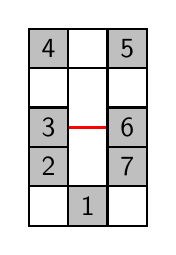
\begin{tikzpicture}
[st/.style={
rectangle,
minimum size=.5cm,
node distance=.5cm,
inner sep = 0cm,
draw=black,thick,fill=#1!50,
font=\sffamily
},
st/.default=gray]
\node (15)[st                   ] {4}; \node (25) [st=white, right of=15] { }; \node (35) [st,       right of= 25] {5};
    \node (14)[st=white,below of= 15] { };                                         \node (34) [st=white, below of= 35] { };
    \node (13)[st,      below of= 14] {3};                                         \node (33) [st,       below of= 34] {6};
    \node (12)[st,      below of= 13] {2};                                         \node (32) [st,       below of= 33] {7};
    \node (11)[st=white,below of= 12] { }; \node (21) [st,       right of=11] {1}; \node (31) [st=white, right of= 21] { };
    \draw[very thick, color=red] (13.east) -- (33.west);

  \end{tikzpicture}
\caption{\textsf{WHITE}}

\end{subfigure}
\hfill
\begin{subfigure}{0.15\textwidth}
\centering
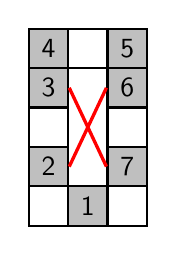
\begin{tikzpicture}
[st/.style={
rectangle,
minimum size=.5cm,
node distance=.5cm,
inner sep = 0cm,
draw=black,thick,fill=#1!50,
font=\sffamily
},
st/.default=gray]
\node (15)[st,                  ] {4}; \node (25) [st=white, right of=15] { }; \node (35) [st,       right of= 25] {5};
    \node (14)[st,      below of= 15] {3};                                         \node (34) [st,       below of= 35] {6};
    \node (13)[st=white,below of= 14] { };                                         \node (33) [st=white, below of= 34] { };
    \node (12)[st,      below of= 13] {2};                                         \node (32) [st,       below of= 33] {7};
    \node (11)[st=white,below of= 12] { }; \node (21) [st,       right of=11] {1}; \node (31) [st=white, right of= 21] { };
    
    \draw[very thick, color=red] (14.east) -- (32.west);
    \draw[very thick, color=red] (12.east) -- (34.west);

  \end{tikzpicture}
\caption{\textsf{BLUE}}

\end{subfigure}
\hfill
\begin{subfigure}{0.15\textwidth}
\centering
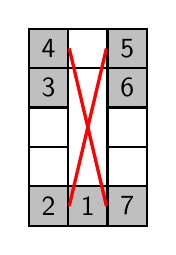
\begin{tikzpicture}
[st/.style={
rectangle,
minimum size=.5cm,
node distance=.5cm,
inner sep = 0cm,
draw=black,thick,fill=#1!50,
font=\sffamily
},
st/.default=gray]
\node (15)[st,                  ] {4}; \node (25) [st=white, right of=15] { }; \node (35) [st,       right of =25] {5};
  \node (14)[st,      below of= 15] {3};                                         \node (34) [st,       below of =35] {6};
  \node (13)[st=white,below of= 14] { };                                         \node (33) [st=white, below of =34] { };
  \node (12)[st=white,below of= 13] { };                                         \node (32) [st=white, below of =33] { };
  \node (11)[st,      below of= 12] {2}; \node (21) [st,       right of=11] {1}; \node (31) [st,       right of =21] {7};

  \draw[very thick, color=red] (15.east) -- (31.west);
  \draw[very thick, color=red] (11.east) -- (35.west);

\end{tikzpicture}   
\caption{\textsf{RED}}

\end{subfigure}
\hfill
\begin{subfigure}{0.15\textwidth}
\centering
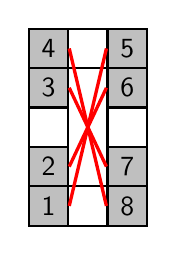
\begin{tikzpicture}
[st/.style={
rectangle,
minimum size=.5cm,
node distance=.5cm,
inner sep = 0cm,
draw=black,thick,fill=#1!50,
font=\sffamily
},
st/.default=gray]
\node (15)[st,                  ] {4}; \node (25) [st=white, right of=15] { }; \node (35) [st,       right of =25] {5};
  \node (14)[st,      below of= 15] {3};                                         \node (34) [st,       below of =35] {6};
  \node (13)[st=white,below of= 14] { };                                         \node (33) [st=white, below of =34] { };
  \node (12)[st      ,below of= 13] {2};                                         \node (32) [st,       below of =33] {7};
  \node (11)[st,      below of= 12] {1}; \node (21) [st=white, right of=11] { }; \node (31) [st,       right of =21] {8};
  
  \draw[very thick, color=red] (15.east) -- (31.west);
  \draw[very thick, color=red] (11.east) -- (35.west);
  \draw[very thick, color=red] (14.east) -- (32.west);
  \draw[very thick, color=red] (12.east) -- (34.west);      

\end{tikzpicture}    
\caption{\textsf{BLACK}}

\end{subfigure}
\hfill
\begin{subfigure}{0.15\textwidth}
\centering
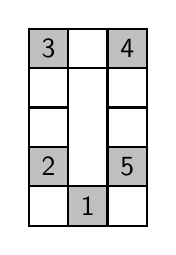
\begin{tikzpicture}
[st/.style={
rectangle,
minimum size=.5cm,
node distance=.5cm,
inner sep = 0cm,
draw=black,thick,fill=#1!50,
font=\sffamily
},
st/.default=gray]
\node (15)[st                   ] {3}; \node (25) [st=white, right of=15] { }; \node (35) [st,       right of= 25] {4};
  \node (14)[st=white,below of= 15] { };                                         \node (34) [st=white, below of= 35] { };
  \node (13)[st=white,below of= 14] { };                                         \node (33) [st=white, below of= 34] { };
  \node (12)[st,      below of= 13] {2};                                         \node (32) [st,       below of= 33] {5};
  \node (11)[st=white,below of= 12] { }; \node (21) [st,       right of=11] {1}; \node (31) [st=white, right of= 21] { };

\end{tikzpicture}    
\caption{\textsf{PENTA}}

\end{subfigure}
\hfill
\begin{subfigure}{0.15\textwidth}
\centering
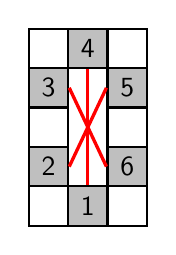
\begin{tikzpicture}
[st/.style={
rectangle,
minimum size=.5cm,
node distance=.5cm,
inner sep = 0cm,
draw=black,thick,fill=#1!50,
font=\sffamily
},
st/.default=gray]
\node (15)[st=white             ] { }; \node (25) [st,       right of=15] {4}; \node (35) [st=white, right of= 25] { };
  \node (14)[st,      below of= 15] {3};                                         \node (34) [st,       below of= 35] {5};
  \node (13)[st=white,below of= 14] { };                                         \node (33) [st=white, below of= 34] { };
  \node (12)[st,      below of= 13] {2};                                         \node (32) [st,       below of= 33] {6};
  \node (11)[st=white,below of= 12] { }; \node (21) [st,       right of=11] {1}; \node (31) [st=white, right of= 21] { };
\draw[ very thick, color=red] (21.north)-- (25.south);
  \draw[ very thick, color=red] (12.east) -- (34.west);
  \draw[very thick, color=red] (14.east) -- (32.west);

\end{tikzpicture}    
\caption{\textsf{TONES}}

\end{subfigure}
\hfill
\caption{The six scales and their tritones}\label{fig:the-six-scales-and-tritones}
\end{figure}
As you can see, the \texttt{WHITE} scale (diatonic major scale, the most used in classical music) only has one tritone.
The \texttt{BLUE} scale (remember, in standard terminology, \emph{melodic minor}) is, by far, the most used in jazz. It has two tritones and this allows for greater capacity for deception and surprise, varying almost imperceptibly between major/minor and minor/major sensations.
The \texttt{RED} scale is widely used in flamenco, also with two tritones.
The \texttt{BLACK} scale has 4 tritones, it is used a lot in classical music when you want to emphasize the tritone sensation, without palliatives or tricks, it does not offer any space for relaxation and is usually used for short periods of time.
The \texttt{PENTA} scale does not have any tritone. There are no threats, it is used in simple music, children's songs or basically in all primitive civilizations. There is no possibility of deception or surprise and it does not ask the listener any questions. It is rather decorative, suitable for the adornment of parties and primary expressions. Its triads give rise to a type of harmony called \emph{fourths harmony}.
The \texttt{TONES} scale has three tritones, but only six notes and also, it has no possible orientation. We will talk about this later.
This same thing happens with \texttt{BLUE} and \texttt{RED}, although there are two tritones.
However, in \texttt{BLACK} we find eight notes in the scale, so between each note of the tritone there are always three, no matter in what direction we move.
The same thing happens with \texttt{TONES}, although there are only two notes in each direction, so by alternating jumps we can never complete a tritone.
The feeling for the listener that the stack that is sounding is close to or far from the tritone must always be counted upwards, that is, how many alternate notes must be added so that a tritone ends up sounding (if it ever happens).
\subsection{Tritonal sense}
It is important to observe that the situation of the tritones has a sense, that is, it may not be the same to go from one note to another by changing the starting note, that depends on whether there are the same notes between the two by both paths. We see that in \texttt{WHITE}, going from degree 6 to degree 3, stacking alternate notes, we would form the chord 6 1 3. However, to go from 3 to 6 we would stack 3, 5, 7, 2, 4, 6. That is, degree 3 is much further away from having a tritone than degree 6, specifically, four levels of stacking further away.
\subsection{Tonal center}
We will call the \emph{tonal center} the central note of the scale. In all of them, it is the note that maintains the same distance with all the tritones by both paths, descending and ascending. It is the most stable degree of all. Do not confuse it with the one that offers a greater sense of relaxation, that is the one that is farthest from some tritone. The central note does not give a feeling of relaxation, but of balance. We could say that it is the most \emph{neutral} degree of the scale. In the \texttt{BLACK} scale, there is no note that occupies that tonal center, although it is perfectly symmetrical, like the others.
\subsection{Ambiguous thirds}
Some scales have an ambiguous third on one of their degrees, that is, it could be a major third or also a minor third. This greatly expands the possibilities for deception and surprise, and is a great help for \emph{modulation} which consists of changing tonality, that is, selecting another scale.
\begin{figure}
\begin{subfigure}{0.15\textwidth}
\centering
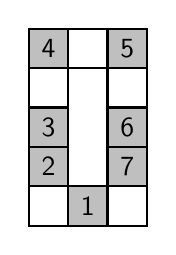
\begin{tikzpicture}
[st/.style={
rectangle,
minimum size=.5cm,
node distance=.5cm,
inner sep = 0cm,
draw=black,thick,fill=#1!50,
font=\sffamily
},
st/.default=gray]
\node (15)[st                   ] {4}; \node (25) [st=white, right of=15] { }; \node (35) [st,       right of= 25] {5};
    \node (14)[st=white,below of= 15] { };                                         \node (34) [st=white, below of= 35] { };
    \node (13)[st,      below of= 14] {3};                                         \node (33) [st,       below of= 34] {6};
    \node (12)[st,      below of= 13] {2};                                         \node (32) [st,       below of= 33] {7};
    \node (11)[st=white,below of= 12] { }; \node (21) [st,       right of=11] {1}; \node (31) [st=white, right of= 21] { };

  \end{tikzpicture}
\caption{\textsf{WHITE}}

\end{subfigure}
\hfill
\begin{subfigure}{0.15\textwidth}
\centering
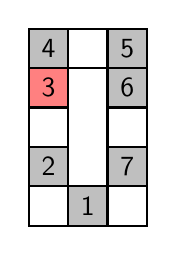
\begin{tikzpicture}
[st/.style={
rectangle,
minimum size=.5cm,
node distance=.5cm,
inner sep = 0cm,
draw=black,thick,fill=#1!50,
font=\sffamily
},
st/.default=gray]
\node (15)[st,                  ] {4}; \node (25) [st=white, right of=15] { }; \node (35) [st,       right of= 25] {5};
    \node (14)[st=red,  below of= 15] {3};                                         \node (34) [st,       below of= 35] {6};
    \node (13)[st=white,below of= 14] { };                                         \node (33) [st=white, below of= 34] { };
    \node (12)[st,      below of= 13] {2};                                         \node (32) [st,       below of= 33] {7};
    \node (11)[st=white,below of= 12] { }; \node (21) [st,       right of=11] {1}; \node (31) [st=white, right of= 21] { };
    
  \end{tikzpicture}
\caption{\textsf{BLUE}}

\end{subfigure}
\hfill
\begin{subfigure}{0.15\textwidth}
\centering
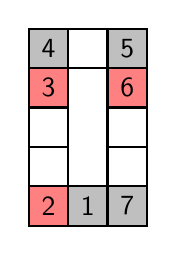
\begin{tikzpicture}
[st/.style={
rectangle,
minimum size=.5cm,
node distance=.5cm,
inner sep = 0cm,
draw=black,thick,fill=#1!50,
font=\sffamily
},
st/.default=gray]
\node (15)[st,                  ] {4}; \node (25) [st=white, right of=15] { }; \node (35) [st,       right of =25] {5};
  \node (14)[st=red,  below of= 15] {3};                                         \node (34) [st=red,   below of =35] {6};
  \node (13)[st=white,below of= 14] { };                                         \node (33) [st=white, below of =34] { };
  \node (12)[st=white,below of= 13] { };                                         \node (32) [st=white, below of =33] { };
  \node (11)[st=red,  below of= 12] {2}; \node (21) [st,       right of=11] {1}; \node (31) [st,       right of =21] {7};

\end{tikzpicture}   
\caption{\textsf{RED}}

\end{subfigure}
\hfill
\begin{subfigure}{0.15\textwidth}
\centering
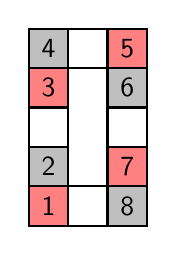
\begin{tikzpicture}
[st/.style={
rectangle,
minimum size=.5cm,
node distance=.5cm,
inner sep = 0cm,
draw=black,thick,fill=#1!50,
font=\sffamily
},
st/.default=gray]
\node (15)[st,                  ] {4}; \node (25) [st=white, right of=15] { }; \node (35) [st=red,   right of =25] {5};
  \node (14)[st=red,  below of= 15] {3};                                         \node (34) [st,       below of =35] {6};
  \node (13)[st=white,below of= 14] { };                                         \node (33) [st=white, below of =34] { };
  \node (12)[st      ,below of= 13] {2};                                         \node (32) [st=red,   below of =33] {7};
  \node (11)[st=red,  below of= 12] {1}; \node (21) [st=white, right of=11] { }; \node (31) [st,       right of =21] {8};

\end{tikzpicture}    
\caption{\textsf{BLACK}}

\end{subfigure}
\hfill
\begin{subfigure}{0.15\textwidth}
\centering
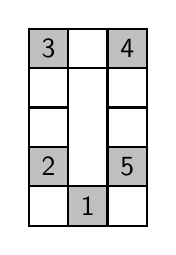
\begin{tikzpicture}
[st/.style={
rectangle,
minimum size=.5cm,
node distance=.5cm,
inner sep = 0cm,
draw=black,thick,fill=#1!50,
font=\sffamily
},
st/.default=gray]
\node (15)[st                   ] {3}; \node (25) [st=white, right of=15] { }; \node (35) [st,       right of= 25] {4};
  \node (14)[st=white,below of= 15] { };                                         \node (34) [st=white, below of= 35] { };
  \node (13)[st=white,below of= 14] { };                                         \node (33) [st=white, below of= 34] { };
  \node (12)[st,      below of= 13] {2};                                         \node (32) [st,       below of= 33] {5};
  \node (11)[st=white,below of= 12] { }; \node (21) [st,       right of=11] {1}; \node (31) [st=white, right of= 21] { };

\end{tikzpicture}    
\caption{\textsf{PENTA}}

\end{subfigure}
\hfill
\begin{subfigure}{0.15\textwidth}
\centering
\begin{tikzpicture}
[st/.style={
rectangle,
minimum size=.5cm,
node distance=.5cm,
inner sep = 0cm,
draw=black,thick,fill=#1!50,
font=\sffamily
},
st/.default=gray]
\node (15)[st=white             ] { }; \node (25) [st,       right of=15] {4}; \node (35) [st=white, right of= 25] { };
  \node (14)[st,      below of= 15] {3};                                         \node (34) [st,       below of= 35] {5};
  \node (13)[st=white,below of= 14] { };                                         \node (33) [st=white, below of= 34] { };
  \node (12)[st,      below of= 13] {2};                                         \node (32) [st,       below of= 33] {6};
  \node (11)[st=white,below of= 12] { }; \node (21) [st,       right of=11] {1}; \node (31) [st=white, right of= 21] { };

\end{tikzpicture}    
\caption{\textsf{TONES}}

\end{subfigure}
\hfill
\caption{The six scales and ambiguous thirds}\label{fig:the-six-scales-and-ambiguous-thirds}
\end{figure}
In this scheme we observe (marked in dark) the degrees that form a third that can be major and also minor.
\begin{itemize} \tightlist
\item \texttt{WHITE} is perfectly unambiguous, because all its thirds are major or minor.
\item \texttt{BLUE} has one ambiguity, on its third degree
\item \texttt{RED} has three: second, third and sixth.
\item \texttt{BLACK} has four on alternate notes, first, third, fifth and seventh.
\item \texttt{PENTA} has no ambiguity: it is direct, clear and simple.
\item \texttt{TONES} has no ambiguity, because all its thirds are major, but this generates a weak capacity for orientation: the listener will not be able to easily detect what degree of the scale we are on.
\end{itemize}
The feeling of ambiguity between the major/minor character of a triad produces uneasiness in the listener, and it is a kind of guessing game that requires attentive and active listening. The map is not clear, and the path is labyrinthine, besides there are many surprises waiting at each crossing. You need a specific attitude to listen to music with many ambiguities. Jazz makes extensive use of ambiguity.
\subsection{Absence of thirds}
If all the degrees of the scale have a third, major or minor, we will consider that, at least in that respect, it is complete. We can observe that in the \texttt{RED} scale there is a degree that does not have any kind of third: the seventh, as well as in the \texttt{PENTA} scale two thirds are missing, on the first and third degrees.
\begin{figure}[H]
\centering
\begin{subfigure}{0.15\textwidth}
\centering
\begin{tikzpicture}
[st/.style={
rectangle,
minimum size=.5cm,
node distance=.5cm,
inner sep = 0cm,
draw=black,thick,fill=#1!50,
font=\sffamily
},
st/.default=gray]
\node (15)[st,                  ] {4}; \node (25) [st=white, right of=15] { }; \node (35) [st,       right of =25] {5};
  \node (14)[st,      below of= 15] {3};                                         \node (34) [st,       below of =35] {6};
  \node (13)[st=white,below of= 14] { };                                         \node (33) [st=white, below of =34] { };
  \node (12)[st=white,below of= 13] { };                                         \node (32) [st=white, below of =33] { };
  \node (11)[st,      below of= 12] {2}; \node (21) [st,       right of=11] {1}; \node (31) [st=red,   right of =21] {7};

\end{tikzpicture}    
\caption{\textsf{RED}}

\end{subfigure}
\begin{subfigure}{0.15\textwidth}
\centering
\begin{tikzpicture}
[st/.style={
rectangle,
minimum size=.5cm,
node distance=.5cm,
inner sep = 0cm,
draw=black,thick,fill=#1!50,
font=\sffamily
},
st/.default=gray]
\node (15)[st=red               ] {3}; \node (25) [st=white, right of=15] { }; \node (35) [st,       right of= 25] {4};
  \node (14)[st=white,below of= 15] { };                                         \node (34) [st=white, below of= 35] { };
  \node (13)[st=white,below of= 14] { };                                         \node (33) [st=white, below of= 34] { };
  \node (12)[st,      below of= 13] {2};                                         \node (32) [st,       below of= 33] {5};
  \node (11)[st=white,below of= 12] { }; \node (21) [st=red,   right of=11] {1}; \node (31) [st=white, right of= 21] { };

\end{tikzpicture}    
\caption{\textsf{PENTA}}

\end{subfigure}
\hfill
\caption{Scales with degrees without thirds}\label{fig:scales-with-no-thirds}
\end{figure}
\subsection{Distances to tritones}
If there are tritones in a scale, each triad will be at a distance from them. The distance represents for the listener the probability that, by adding more notes to the chord, they will hear a tritone. It is easy to appreciate in this scheme of the \texttt{WHITE} scale that the two triads farthest from the tritone are, on the one hand the triad \texttt{CEG} and on the other \texttt{ACE}.
It turns out that in standard notation, these triads are called \emph{fundamental degree} and \emph{relative minor}. Besides the outlandish nomenclature, they are the degrees that are used to begin and end most of the themes. They simply suggest rest and stability, although one is major and the other is minor, so they also have their own character. If it ends on a chord close to the tritone, probably no one will applaud: there is unresolved tension, unanswered questions.
\begin{figure}[H]
\centering
\begin{subfigure}{1\textwidth}
\centering
\begin{tikzpicture}
[st/.style={
rectangle,
minimum size=.4cm,
node distance=0cm,
inner sep = 0cm,
draw=black,thick,fill=#1!50,
font=\sffamily
},
st/.default=white]
\node (1)  [st]              {C};
  \node (2)  [st, right=of 1]  { };
  \node (3)  [st, right=of 2]  { };
  \node (4)  [st, right=of 3]  { };
  \node (5)  [st, right=of 4]  {E};
  \node (6)  [st, right=of 5]  { };
  \node (7)  [st, right=of 6]  { };
  \node (8)  [st, right=of 7]  {G};
  \node (9)  [st, right=of 8]  { };
  \node (10) [st, right=of 9]  { };
  \node (11) [st, right=of 10] { };
  \node (12) [st=gray, right=of 11] {B};
  \node (13) [st, right=of 12] { };
  \node (14) [st, right=of 13] { };
  \node (15) [st, right=of 14] {D};
  \node (16) [st, right=of 15] { };
  \node (17) [st, right=of 16] { };
  \node (18) [st=gray, right=of 17] {F};
  \node (19) [st, right=of 18] { };
  \node (20) [st, right=of 19] { };
  \node (21) [st, right=of 20] { };
  \node (22) [st, right=of 21] {A};
  \node (23) [st, right=of 22] { };
  \node (24) [st, right=of 23] { };
  \node (25) [st, right=of 24] {C};
  \node (26) [st, right=of 25] { };
  \node (27) [st, right=of 26] { };
  \node (28) [st, right=of 27] { };
  \node (29) [st, right=of 28] {E};

  \draw [ultra thick, color=red] (12.north) to [out=45,in=135] (18.north);

  \node (t1-C) [st, draw=none, below=3pt of 1]  { };
  \node (t1-E) [st, draw=none, below=3pt of 5]  {E};
  \node (t1-G) [st, draw=none, below=3pt of 8]  {G};
  \node (t1-B) [st, draw=none, below=3pt of 12] {B};

  \node (t2-D) [st, draw=none, below=3pt of 15] { };
  \node (t2-F) [st, draw=none, below=3pt of 18] {F};
  \node (t2-A) [st, draw=none, below=3pt of 22] {A};
  \node (t2-C) [st, draw=none, below=3pt of 25] {C};
  \node (t2-E) [st, draw=none, below=3pt of 29] { };
  
  \draw [rounded corners=2mm] (t1-E.north west) rectangle (t1-B.south east);
  \draw [rounded corners=2mm] (t2-F.north west) rectangle (t2-C.south east);

  \node (t3-C) [st, draw=none, below=3pt of t1-C] { };
  \node (t3-E) [st, draw=none, below=3pt of t1-E] { };
  \node (t3-G) [st, draw=none, below=3pt of t1-G] {G};
  \node (t3-B) [st, draw=none, below=3pt of t1-B] {B};
  \node (t4-D) [st, draw=none, below=3pt of t2-D] {D};
  \node (t4-F) [st, draw=none, below=3pt of t2-F] {F};
  \node (t4-A) [st, draw=none, below=3pt of t2-A] {A};
  \node (t4-C) [st, draw=none, below=3pt of t2-C] { };
  \node (t4-E) [st, draw=none, below=3pt of t2-E] { };
  
  \draw [rounded corners=2mm] (t3-G.north west) rectangle (t4-D.south east);
  \draw [rounded corners=2mm] (t4-D.north west) rectangle (t4-A.south east);

  \node (t5-C) [st, draw=none, below=3pt of t3-C] {C};
  \node (t5-E) [st, draw=none, below=3pt of t3-E] {E};
  \node (t5-G) [st, draw=none, below=3pt of t3-G] {G};
  \node (t6-B) [st, draw=none, below=3pt of t3-B] {B};
  \node (t6-D) [st, draw=none, below=3pt of t4-D] {D};
  \node (t6-F) [st, draw=none, below=3pt of t4-F] {F};
  \node (t7-A) [st, draw=none, below=3pt of t4-A] {A};
  \node (t7-C) [st, draw=none, below=3pt of t4-C] {C};
  \node (t7-E) [st, draw=none, below=3pt of t4-E] {E};

  \draw [rounded corners=2mm] (t5-C.north west) rectangle (t5-G.south east);
  \draw [rounded corners=2mm] (t6-B.north west) rectangle (t6-F.south east);
  \draw [rounded corners=2mm] (t7-A.north west) rectangle (t7-E.south east);
\end{tikzpicture}

\end{subfigure}
\caption{Scale \textsf{WHITE} with its triads}\label{fig:white-scale-with-its-triads}
\end{figure}
In this other figure we observe the \texttt{BLUE} scale, with its two tritones and the corresponding triads. We see that there is no triad that is sufficiently far away from a tritone, when we move away from one we get closer to the other. You can see that the triads that are ``safest'' seem to be \texttt{CeG}, which would need to add \texttt{B}, \texttt{D} and \texttt{F} to contain a tritone, also \texttt{DFA} which would need to add \texttt{C} and \texttt{e} for the same thing, and \texttt{eGB} which would need \texttt{D} and \texttt{F}.
It is not a very comfortable scale, for this reason: when we reach a degree it gives the impression that we still need to get out of there somehow. In standard terminology, they talk about \emph{tension}. It is a suitable term if we understand it as \emph{unanswered question}. In no case should we think of something unpleasant or repellent, it is just music.
\begin{figure}[H]
\centering
\begin{subfigure}{1\textwidth}
\centering
\begin{tikzpicture}
[st/.style={
rectangle,
minimum size=.4cm,
node distance=0cm,
inner sep = 0cm,
draw=black,thick,fill=#1!50,
font=\sffamily
},
st/.default=white]
\node (1)  [st]              {F};
  \node (2)  [st, right=of 1]  { };
  \node (3)  [st, right=of 2]  { };
  \node (4)  [st, right=of 3]  { };
  \node (5)  [st=gray, right=of 4]  {A};
  \node (6)  [st, right=of 5]  { };
  \node (7)  [st, right=of 6]  { };
  \node (8)  [st, right=of 7]  {C};
  \node (9)  [st, right=of 8]  { };
  \node (10) [st, right=of 9]  { };
  \node (11) [st=gray, right=of 10] {e};
  \node (12) [st, right=of 11] { };
  \node (13) [st, right=of 12] { };
  \node (14) [st, right=of 13] { };
  \node (15) [st, right=of 14] {G};
  \node (16) [st, right=of 15] { };
  \node (17) [st, right=of 16] { };
  \node (18) [st, right=of 17] { };
  \node (19) [st=gray, right=of 18] {B};
  \node (20) [st, right=of 19] { };
  \node (21) [st, right=of 20] { };
  \node (22) [st, right=of 21] {D};
  \node (23) [st, right=of 22] { };
  \node (24) [st, right=of 23] { };
  \node (25) [st=gray, right=of 24] {F};
  \node (26) [st, right=of 25] { };
  \node (27) [st, right=of 26] { };
  \node (28) [st, right=of 27] { };
  \node (29) [st, right=of 28] {A};

  \draw [ultra thick, color=red] (5.north) to [out=45,in=135] (11.north);
  \draw [ultra thick, color=red] (19.north) to [out=45,in=135] (25.north);

  \node (t1-F) [st, draw=none, below=3pt of 1]  { };
  \node (t1-A) [st, draw=none, below=3pt of 5]  {A};
  \node (t1-C) [st, draw=none, below=3pt of 8]  {C};
  \node (t1-e) [st, draw=none, below=3pt of 11] {e};

  \node (t2-G) [st, draw=none, below=3pt of 15] { };
  \node (t2-B) [st, draw=none, below=3pt of 19] {B};
  \node (t2-D) [st, draw=none, below=3pt of 22] {D};
  \node (t2-F) [st, draw=none, below=3pt of 25] {F};
  \node (t2-A) [st, draw=none, below=3pt of 29] { };
  
  \draw [rounded corners=2mm] (t1-A.north west) rectangle (t1-e.south east);
  \draw [rounded corners=2mm] (t2-B.north west) rectangle (t2-F.south east);

  \node (t3-F) [st, draw=none, below=3pt of t1-F] { };
  \node (t3-A) [st, draw=none, below=3pt of t1-A] { };
  \node (t3-C) [st, draw=none, below=3pt of t1-C] {C};
  \node (t3-e) [st, draw=none, below=3pt of t1-e] {e};
  \node (t4-G) [st, draw=none, below=3pt of t2-G] {G};
  \node (t4-B) [st, draw=none, below=3pt of t2-B] {B};
  \node (t4-D) [st, draw=none, below=3pt of t2-D] {D};
  \node (t4-F) [st, draw=none, below=3pt of t2-F] { };
  \node (t4-A) [st, draw=none, below=3pt of t2-A] { };
  
  \draw [rounded corners=2mm] (t3-C.north west) rectangle (t4-G.south east);
  \draw [rounded corners=2mm] (t4-G.north west) rectangle (t4-D.south east);

  \node (t5-F) [st, draw=none, below=3pt of t3-F] {F};
  \node (t5-A) [st, draw=none, below=3pt of t3-A] {A};
  \node (t5-C) [st, draw=none, below=3pt of t3-C] {C};
  \node (t6-e) [st, draw=none, below=3pt of t3-e] {e};
  \node (t6-G) [st, draw=none, below=3pt of t4-G] {G};
\node (t6-B) [st, draw=none, below=3pt of t4-B] {B};
\node (t7-D) [st, draw=none, below=3pt of t4-D] {D};
\node (t7-F) [st, draw=none, below=3pt of t4-F] {F};
\node (t7-A) [st, draw=none, below=3pt of t4-A] {A};
\draw [rounded corners=2mm] (t5-F.north west) rectangle (t5-C.south east);
  \draw [rounded corners=2mm] (t6-e.north west) rectangle (t6-B.south east);
  \draw [rounded corners=2mm] (t7-D.north west) rectangle (t7-A.south east);
\end{tikzpicture}

\end{subfigure}
\caption{Scale \textsf{BLUE} with its triads}\label{fig:blue-scale-with-its-triads}
\end{figure}
\subsection{Are there no more scales?}
Looking for more is an interesting exercise. It would be fantastic to find some, but the properties we have seen so far restrict the possibilities.
\begin{itemize} \tightlist
\item Whether or not there are tritones
\item Whether all degrees have a third or not
\item Whether all the thirds are major or minor
\item That they form a symmetrical combination
\item That the orientation is unique
\item That the notes are distributed without being grouped into blocks
\end{itemize}
Any combination that is found will simply be a different ordering of one of the six presented (which would be a mode, remember). If you rotate it in the scheme you will get to it. Let's try a few:
\begin{figure}[H]
\begin{subfigure}{0.15\textwidth}
\centering
\begin{tikzpicture}
[st/.style={
rectangle,
minimum size=.5cm,
node distance=.5cm,
inner sep = 0cm,
draw=black,thick,fill=#1!50,
font=\sffamily
},
st/.default=gray]
\node (15)[st                   ] {4}; \node (25) [st=white, right of=15] { }; \node (35) [st,       right of= 25] {5};
    \node (14)[st=white,below of= 15] { };                                         \node (34) [st=white, below of= 35] { };
    \node (13)[st,      below of= 14] {3};                                         \node (33) [st,       below of= 34] {6};
    \node (12)[st=white,below of= 13] { };                                         \node (32) [st=white, below of= 33] { };
    \node (11)[st,      below of= 12] {2}; \node (21) [st,       right of=11] {1}; \node (31) [st,       right of= 21] {7};

  \end{tikzpicture}
\caption{\textsf{X1}}

\end{subfigure}
\hfill
\begin{subfigure}{0.15\textwidth}
\centering
\begin{tikzpicture}
[st/.style={
rectangle,
minimum size=.5cm,
node distance=.5cm,
inner sep = 0cm,
draw=black,thick,fill=#1!50,
font=\sffamily
},
st/.default=gray]
\node (15)[st,                  ] {4}; \node (25) [st=white, right of=15] { }; \node (35) [st,       right of= 25] {5};
    \node (14)[st=white,below of= 15] { };                                         \node (34) [st=white, below of= 35] { };
    \node (13)[st=white,below of= 14] { };                                         \node (33) [st=white, below of= 34] { };
    \node (12)[st,      below of= 13] {3};                                         \node (32) [st,       below of= 33] {6};
    \node (11)[st,      below of= 12] {2}; \node (21) [st,       right of=11] {1}; \node (31) [st,       right of= 21] {7};

  \end{tikzpicture}
\caption{\textsf{X2}}

\end{subfigure}
\hfill
\begin{subfigure}{0.15\textwidth}
\centering
\begin{tikzpicture}
[st/.style={
rectangle,
minimum size=.5cm,
node distance=.5cm,
inner sep = 0cm,
draw=black,thick,fill=#1!50,
font=\sffamily
},
st/.default=gray]
\node (15)[st,                  ] {4}; \node (25) [st=white, right of=15] { }; \node (35) [st,       right of =25] {5};
  \node (14)[st=white,below of= 15] { };                                         \node (34) [st=white, below of =35] { };
  \node (13)[st,      below of= 14] {3};                                         \node (33) [st,       below of =34] {6};
  \node (12)[st,      below of= 13] {2};                                         \node (32) [st,       below of =33] {7};
  \node (11)[st,      below of= 12] {1}; \node (21) [st=white, right of=11] { }; \node (31) [st,       right of =21] {8};

\end{tikzpicture}    
\caption{\textsf{X3}}

\end{subfigure}
\hfill
\begin{subfigure}{0.15\textwidth}
\centering
\begin{tikzpicture}
[st/.style={
rectangle,
minimum size=.5cm,
node distance=.5cm,
inner sep = 0cm,
draw=black,thick,fill=#1!50,
font=\sffamily
},
st/.default=gray]
\node (15)[st=white,            ] { }; \node (25) [st, right of=15] {4}; \node (35)       [st=white, right of =25] { };
  \node (14)[st=white,below of= 15] { };                                         \node (34) [st=white, below of =35] { };
  \node (13)[st,      below of= 14] {3};                                         \node (33) [st,       below of =34] {5};
  \node (12)[st      ,below of= 13] {2};                                         \node (32) [st,       below of =33] {6};
  \node (11)[st=white,below of= 12] { }; \node (21) [st, right of=11] {1}; \node (31)       [st=white, right of =21] { };

\end{tikzpicture}   
\caption{\textsf{X4}}

\end{subfigure}
\hfill
\begin{subfigure}{0.15\textwidth}
\centering
\begin{tikzpicture}
[st/.style={
rectangle,
minimum size=.5cm,
node distance=.5cm,
inner sep = 0cm,
draw=black,thick,fill=#1!50,
font=\sffamily
},
st/.default=gray]
\node (15)[st                   ] {3}; \node (25) [st,       right of=15] {4}; \node (35) [st,       right of= 25] {5};
  \node (14)[st=white,below of= 15] { };                                         \node (34) [st=white, below of= 35] { };
  \node (13)[st=white,below of= 14] { };                                         \node (33) [st=white, below of= 34] { };
  \node (12)[st=white,below of= 13] { };                                         \node (32) [st=white, below of= 33] { };
  \node (11)[st,      below of= 12] {2}; \node (21) [st,       right of=11] {1}; \node (31) [st,       right of= 21] {6};

\end{tikzpicture}    
\caption{\textsf{X5}}

\end{subfigure}
\hfill
\caption{Other possible scales}\label{fig:more-posible-scales}
\end{figure}
\begin{table}[H]
\centering
\begin{tabular}{lccc}
\toprule
Scale & Ambiguous thirds & No third & Tritones \\
\midrule
X1 & 1 & 0 & 3 \\
X2 & 2 & 2 & 2 \\
X3 & 3 & 1 & 3 \\
X4 & 1 & 0 & 2 \\
X5 & 0 & 6 & 3 \\
\bottomrule
\end{tabular}
\caption{Characteristics of different musical scales}\label{tab:escalas}
\end{table}
\subsection{Order of triads by distances to the tritones}
In these two scales \texttt{WHITE} and \texttt{BLUE} the shaded tritones are appreciated. The first has one: \texttt{B-F}, and the second has two: \texttt{A-e} and \texttt{B-F}. To modulate between one and the other, simply change the note \texttt{E} for \texttt{e} (\texttt{Mi} for \texttt{Mi flat}). The symmetrical center was the note \texttt{D} in \texttt{WHITE} and now it becomes \texttt{G} in \texttt{BLUE}.
Let's look at all the triads of the scale and the distance they keep with the next tritone, that is, the number of thirds that would have to be added to it so that it contains a tritone. We will also note if the triad already includes any note belonging to some tritone. The distance that the listener perceives is what decides whether the triad can be considered the safe target of a resolution.
For the moment, we do not have a mathematical formula that allows us to calculate this force, but it seems clear that the triads considered as rest'' in which the melody mustresolve'' are the ones that are farthest from containing a tritone. In the case of \textsf{WHITE}, the triads \textsf{ACE} and \textsf{CEG}, also called tonics'', one minor and the other major. Only \textsf{DFA} is at the same distance, but it already contains a note from the tritone ( \textsf{F} ) which makes it lesssafe''.
\begin{figure}[H]
\centering
\begin{subfigure}{1\textwidth}
\centering
\begin{tikzpicture}
[st/.style={
rectangle,
minimum size=.4cm,
node distance=0cm,
inner sep = 0cm,
draw=black,thick,fill=#1!50,
font=\sffamily
},
st/.default=white]
\node (1)  [st=gray]         {F};
  \node (2)  [st, right=of 1]  { };
  \node (3)  [st, right=of 2]  { };
  \node (4)  [st, right=of 3]  { };
  \node (5)  [st, right=of 4]  {A};
  \node (6)  [st, right=of 5]  { };
  \node (7)  [st, right=of 6]  { };
  \node (8)  [st, right=of 7]  {C};
  \node (9)  [st, right=of 8]  { };
  \node (10) [st, right=of 9]  { };
  \node (11) [st, right=of 10] { };
  \node (12) [st, right=of 11] {E};
  \node (13) [st, right=of 12] { };
  \node (14) [st, right=of 13] { };
  \node (15) [st, right=of 14] {G};
  \node (16) [st, right=of 15] { };
  \node (17) [st, right=of 16] { };
  \node (18) [st, right=of 17] { };
  \node (19) [st=gray, right=of 18] {B};
  \node (20) [st=gray, right=of 19] { };
  \node (21) [st=gray, right=of 20] { };
  \node (22) [st=gray, right=of 21] {D};
  \node (23) [st=gray, right=of 22] { };
  \node (24) [st=gray, right=of 23] { };
  \node (25) [st=gray, right=of 24] {F};
  \node (26) [st, right=of 25] { };
  \node (27) [st, right=of 26] { };
  \node (28) [st, right=of 27] { };
  \node (29) [st, right=of 28] {A};

\end{tikzpicture}

\end{subfigure}
\caption{Scale \textsf{WHITE} }\label{fig:white-scale-distances}
\end{figure}
\begin{table}[H]
\centering
\begin{tabular}{lcc}
\toprule
TRIAD & Distance to a tritone & Contains \\
\midrule
GBD & 1 & 1 \\
BDF & 0 & 2 \\
DFA & 4 & 1 \\
FAC & 3 & 1 \\
ACE & 4 & 0 \\
CEG & 3 & 0 \\
EGB & 2 & 1 \\
\bottomrule
\end{tabular}
\caption{Table of triads and their characteristics}\label{tab:white-triads}
\end{table}
\begin{figure}[H]
\centering
\begin{subfigure}{1\textwidth}
\centering
\begin{tikzpicture}
[st/.style={
rectangle,
minimum size=.4cm,
node distance=0cm,
inner sep = 0cm,
draw=black,thick,fill=#1!50,
font=\sffamily
},
st/.default=white]
\node (1)  [st=gray]         {F};
  \node (2)  [st, right=of 1]  { };
  \node (3)  [st, right=of 2]  { };
  \node (4)  [st, right=of 3]  { };
  \node (5)  [st=gray, right=of 4]  {A};
  \node (6)  [st=gray, right=of 5]  { };
  \node (7)  [st=gray, right=of 6]  { };
  \node (8)  [st=gray, right=of 7]  {C};
  \node (9)  [st=gray, right=of 8]  { };
  \node (10) [st=gray, right=of 9]  { };
  \node (11) [st=gray, right=of 10] {e};
  \node (12) [st, right=of 11] { };
  \node (13) [st, right=of 12] { };
  \node (14) [st, right=of 13] { };
  \node (15) [st, right=of 14] {G};
  \node (16) [st, right=of 15] { };
  \node (17) [st, right=of 16] { };
  \node (18) [st, right=of 17] { };
  \node (19) [st=gray, right=of 18] {B};
  \node (20) [st=gray, right=of 19] { };
  \node (21) [st=gray, right=of 20] { };
  \node (22) [st=gray, right=of 21] {D};
  \node (23) [st=gray, right=of 22] { };
  \node (24) [st=gray, right=of 23] { };
  \node (25) [st=gray, right=of 24] {F};
  \node (26) [st, right=of 25] { };
  \node (27) [st, right=of 26] { };
  \node (28) [st, right=of 27] { };
  \node (29) [st=gray, right=of 28] {A};

\end{tikzpicture}

\end{subfigure}
\caption{Scale \textsf{BLUE} }\label{fig:blue-scale-distances}
\end{figure}
\begin{table}[H]
\centering
\begin{tabular}{lcc}
\toprule
TRIAD & Distance to a tritone & Contains \\
\midrule
ACe & 0 & 2 \\
CeG & 3 & 1 \\
eGB & 2 & 2 \\
GBD & 1 & 1 \\
BDF & 0 & 2 \\
DFA & 2 & 2 \\
FAC & 2 & 1 \\
\bottomrule
\end{tabular}
\caption{Table of triads and their characteristics}\label{tab:triadas}
\end{table}
\subsection{Chords of each scale}
The chords that are formed from each of the six scales are the same ones that are normally used, but it would be necessary to refer to them without having to use the inconsistent classical names.
A possible notation for naming chords could consist of specifying only three elements:
\begin{itemize}
\item The scale
\item The mode
\item The density
\end{itemize}
With this simple mechanism we could designate any type of chord with only 4 characters.
To designate the scale, the initial of its name would be enough (except for \textsf{BLACK} which could be assigned the \textsf{K}):
\begin{table}[H]
\centering
\begin{tabular}{ll}
\toprule
SCALE & Key \\
\midrule
\textsf{WHITE} & W \\
\textsf{BLUE} & B \\
\textsf{RED} & R \\
\textsf{BLACK} & K \\
\textsf{PENTA} & P \\
\textsf{TONES} & T \\
\bottomrule
\end{tabular}
\caption{Table of scales and their abbreviated keys}\label{tab:scales-and-keys}
\end{table}
For the mode, it would be enough to specify a number, 0 being the mode corresponding to the tritone center and negative or positive numbers indicating the modes that are above or below the central one.
The density would indicate the number of notes in the chord. It could be that 0 indicates a basic triad and 1 a four-note chord, 2 a five-note chord, etc.
We will show the lists of all chords with the different densities for each scale, as well as their equivalent name in classical notation.
\subsection*{Chords of WHITE}
\subsubsection*{3 notes}
\begin{table}[H]
\centering
\begin{tabularx}{\textwidth}{ll>{\raggedright\arraybackslash}Xl}
\toprule
Notation & Traditional Name & Type & Notes \\
\midrule
\textsf{CW-3} & Am & Minor & A C E \\
\textsf{CW-2} & Bm5 & Minor with flat fifth & B D F \\
\textsf{CW-1} & Cmaj & Major & C E G \\
\textsf{CW 0} & Dm & Minor & D F A \\
\textsf{CW+1} & Em & Minor & E G B \\
\textsf{CW+2} & Fmaj & Major & F A C \\
\textsf{CW+3} & Gmaj & Major & G B D \\
\bottomrule
\end{tabularx}
\end{table}
\subsubsection*{4 notes}
\begin{table}[H]
\centering
\begin{tabularx}{\textwidth}{ll>{\raggedright\arraybackslash}Xl}
\toprule
Notation & Traditional Name & Type & Notes \\
\midrule
\textsf{CW-3} 1 & Am7 & Minor seventh & A C E G \\
\textsf{CW-2} 1 & Bm7b5 & Minor seventh flat fifth & B D F A \\
\textsf{CW-1} 1 & Cmaj7 & Major seventh & C E G B \\
\textsf{CW 0} 1 & Dm7 & Minor seventh & D F A C \\
\textsf{CW+1} 1 & Em7 & Minor seventh & E G B D \\
\textsf{CW+2} 1 & Fmaj7 & Major seventh & F A C E \\
\textsf{CW+3} 1 & G7 & Dominant (seventh) & G B D F \\
\bottomrule
\end{tabularx}
\end{table}
\subsubsection*{5 notes}
\begin{table}[H]
\centering
\begin{tabularx}{\textwidth}{ll>{\raggedright\arraybackslash}Xl}
\toprule
Notation & Traditional Name & Type & Notes \\
\midrule
\textsf{CW-3} 2 & Am9 & Minor ninth & A C E G B \\
\textsf{CW-2} 2 & Bm9b5 & Minor ninth with flat fifth & B D F A C \\
\textsf{CW-1} 2 & Cmaj9 & Major ninth & C E G B D \\
\textsf{CW 0} 2 & Dm9 & Minor ninth & D F A C E \\
\textsf{CW+1} 2 & Em9b9 & Minor ninth flat ninth & E G B D F \\
\textsf{CW+2} 2 & Fmaj9 & Major ninth & F A C E G \\
\textsf{CW+3} 2 & G9 & Dominant ninth & G B D F A \\
\bottomrule
\end{tabularx}
\end{table}
\subsection*{Chords of BLUE}
\subsubsection*{3 notes}
\begin{table}[H]
\centering
\begin{tabularx}{\textwidth}{ll>{\raggedright\arraybackslash}Xl}
\toprule
Notation & Traditional Name & Type & Notes \\
\midrule
\textsf{DB-3} & Bm5 & Minor with flat fifth & B D F \\
\textsf{DB-2} & Cm & Minor & C e G \\
\textsf{DB-1} & Dm & Minor & D F A \\
\textsf{DB 0} & e+ & Major with augmented fifth & e G B \\
\textsf{DB+1} & Fmaj & Major & F A C \\
\textsf{DB+2} & Gmaj & Major & G B D \\
\textsf{DB+3} & Am5 & Minor with flat fifth & A C e \\
\bottomrule
\end{tabularx}
\end{table}
\subsubsection*{4 notes}
\begin{table}[H]
\centering
\begin{tabularx}{\textwidth}{ll>{\raggedright\arraybackslash}Xl}
\toprule
Notation & Traditional Name & Type & Notes \\
\midrule
\textsf{DB-3} 1 & Bm7b5 & Minor seventh with flat fifth & B D F A \\
\textsf{DB-2} 1 & Cm Maj7 & Minor seventh major & C e G B \\
\textsf{DB-1} 1 & Dm7 & Minor seventh & D F A C \\
\textsf{DB 0} 1 & e+Maj7 & Major with augmented fifth and major seventh & e G B D \\
\textsf{DB+1} 1 & F7 & Dominant (seventh) & F A C e \\
\textsf{DB+2} 1 & G7 & Dominant (seventh) & G B D F \\
\textsf{DB+3} 1 & Am7b5 & Minor seventh with flat fifth & A C e G \\
\bottomrule
\end{tabularx}
\end{table}
\subsubsection*{5 notes}
\begin{table}[H]
\centering
\begin{tabularx}{\textwidth}{ll>{\raggedright\arraybackslash}Xl}
\toprule
Notation & Traditional Name & Type & Notes \\
\midrule
\textsf{DB-3} 2 & Bm9b5 & Minor ninth with flat fifth & B D F A C \\
\textsf{DB-2} 2 & Cm Maj9 & Minor ninth major & C e G B D \\
\textsf{DB-1} 2 & Dm9 & Minor ninth & D F A C e \\
\textsf{DB 0} 2 & e+Maj9 & Major with augmented fifth and major ninth & e G B D F \\
\textsf{DB+1} 2 & F9 & Dominant ninth & F A C e G \\
\textsf{DB+2} 2 & G9 & Dominant ninth & G B D F A \\
\textsf{DB+3} 2 & Am9b5 & Minor ninth with flat fifth & A C e G B \\
\bottomrule
\end{tabularx}
\end{table}
\subsection*{Chords of RED}
\subsubsection*{3 notes}
\begin{table}[H]
\centering
\begin{tabularx}{\textwidth}{ll>{\raggedright\arraybackslash}Xl}
\toprule
Notation & Traditional Name & Type & Notes \\
\midrule
\textsf{AW-3} & Eb5 & Major with flat fifth & E a b \\
\textsf{AW-2} & F5+ & Major with augmented fifth & F A d \\
\textsf{AW-1} & adis3b5 & Minor with diminished third and flat fifth & a b D \\
\textsf{AW 0} & AM & Major & A d E \\
\textsf{AW+1} & bM & Major & b D F \\
\textsf{AW+2} & dm & Minor & d E a \\
\textsf{AW+3} & Dm & Minor & D F A \\
\bottomrule
\end{tabularx}
\end{table}
\subsubsection*{4 notes}
\begin{table}[H]
\centering
\begin{tabularx}{\textwidth}{ll>{\raggedright\arraybackslash}Xl}
\toprule
Notation & Traditional Name & Type & Notes \\
\midrule
\textsf{AW-3} & Eb57 & Major with flat fifth and seventh & E a b D \\
\textsf{AW-2} & F5+Maj7 & Major with augmented fifth and major seventh & F A d E \\
\textsf{AW-1} & adis3b56 & Minor with diminished third flat fifth and sixth & a b D F \\
\textsf{AW 0} & Amaj7 & Major with major seventh & A d E a \\
\textsf{AW+1} & bmaj7 & Major with major seventh & b D F A \\
\textsf{AW+2} & dm6 & Minor sixth & d E a b \\
\textsf{AW+3} & DmMaj7 & Minor with major seventh & D F A d \\
\bottomrule
\end{tabularx}
\end{table}
\subsubsection*{5 notes}
\begin{table}[H]
\centering
\begin{tabularx}{\textwidth}{ll>{\raggedright\arraybackslash}Xl}
\toprule
Notation & Traditional Name & Type & Notes \\
\midrule
\textsf{AW-3} & Eb57b9 & Major with flat fifth, seventh and flat ninth & E a b D F \\
\textsf{AW-2} & F5+Maj79+ & Major with augmented fifth, major seventh and augmented ninth & F A d E a \\
\textsf{AW-1} & adis3b569 & Minor with diminished third flat fifth sixth and ninth & a b D F b \\
\textsf{AW 0} & Amaj7b9 & Major with major seventh and flat ninth & A d E a b \\
\textsf{AW+1} & bmaj7+9 & Major with major seventh and augmented ninth & b D F A d \\
\textsf{AW+2} & dm6+9 & Minor sixth with augmented ninth & d E a b d \\
\textsf{AW+3} & DmMaj79 & Minor with major seventh and ninth & D F A d E \\
\bottomrule
\end{tabularx}
\end{table}
We leave the issue of notation pending for later. We need to create an efficient notation that allows us to create complete scores, with melodies, rhythms, chords, lyrics, silences, repetitions, indications, etc.
It should be a portable notation and easily interpretable algorithmically, without duplicities, confusions or special rules.
\subsection{Map of the situation}
If a song were a map and each triad were a point, we could consider the position of the tritones as an elevation in the terrain. The slope that is generated around it makes things tend to move away from that point, let's say that it costs us to get close to them.
The listener perceives the sound map as a set of points that maintain a position with respect to that elevation of the terrain. To agree, let's call it \emph{tritone center}.
Now we have two distinct concepts:
\begin{itemize} \tightlist
\item \emph{Tonal center}, remember, the most neutral note of the scale, equidistant from all the tritones and in the symmetrical center of the scale
\item \emph{Tritone centers}, a kind of terrain elevations whose surrounding slope exerts a force that pushes us away from them
\end{itemize}
If we change the position of the tritone center, the listener will feel disoriented: they will have to recalculate where they have to ``run away'' to, looking for some point of reference as quickly as possible or they will lose track of the theme.
By modulating correctly, we can change some of the notes, moving to another scale, but keeping the position of the tritone center, so the feeling of disorientation will be much weaker.
The trick is to change the tonal center without moving the tritone center. But how is that possible? Well, we can simply leave the tritone center we have where it is, but add another one. If the \emph{slope} of the degree we are on (that is, its position with respect to the previous tritone center) remains the same, the listener will not lose their orientation, however, the tonal center will have been changed.
\subsection{Circular notation}
\begin{figure}[H]
\begin{subfigure}{.30\textwidth}
\centering
\begin{tikzpicture}
[
every label/.style={green},
radius=1.25cm
]
\graph [
simple necklace layout,
node sep=0pt,
grow'=up,
node distance=0pt,
nodes={
draw,
circle,
as = ,
minimum size=20pt,
font=\sffamily
}
]
{
1 [as = D]
-- 2 [draw=none]
-- 3 [as = E]
-- 4 [as = F]
-- 5 [draw=none]
-- 6 [as = G]
-- 7 [draw=none]
-- 8 [as = A]
-- 9 [draw=none]
-- 10 [as = B]
-- 11 [as = C]
-- 12 [draw=none]
};
\draw [] (0,39.50pt) circle [radius=28pt];
\draw[ultra thick, color=red] (4) -- (10);
\end{tikzpicture}
\caption{\textsf{WHITE} with its tritone center in red}
\end{subfigure}
\hfill
\begin{subfigure}{0.30\textwidth}
\centering
\begin{tikzpicture}
[every label/.style={green},
    radius=1.25cm
    ]
    \graph [    
      simple necklace layout,
      node sep=0pt, 
      grow'=up,
      node distance=0pt,    
      nodes={
        draw,
        circle, 
        as =  , 
        minimum size=20pt, 
        font=\sffamily 
      }
    ]
    { 
         1  [as = D] 
      -- 2  [as = e]
      -- 3  [draw=none]
      -- 4  [as = F]
      -- 5  [draw=none]
      -- 6  [as = G]
      -- 7  [draw=none]
      -- 8  [as = A]
      -- 9  [draw=none]
      -- 10 [as = B]
      -- 11 [as = C]
      -- 12 [draw=none]
    };
    \draw [] (0,39.50pt) circle [radius=28pt];
    \draw[ultra thick, color=red] (4) -- (10);
    \draw[ultra thick, color=red] (2) -- (8);
  \end{tikzpicture}
\caption{We add a tritone keeping the previous one. Now we are in \textsf{BLUE}}

\end{subfigure}
\hfill
\begin{subfigure}{0.30\textwidth}
\centering
\begin{tikzpicture}
[
every label/.style={green},
radius=1.25cm
]
\graph [
simple necklace layout,
node sep=0pt,
grow'=up,
node distance=0pt,
nodes={
draw,
circle,
as = ,
minimum size=20pt,
font=\sffamily
}
]
{
1 [as = G]
-- 2 [draw=none]
-- 3 [as = A]
-- 4 [draw=none]
-- 5 [as = B]
-- 6 [as = C]
-- 7 [draw=none]
-- 8 [as = D]
-- 9 [as = e]
-- 10 [draw=none]
-- 11 [as = F]
-- 12 [draw=none]
};
\draw [] (0,39.50pt) circle [radius=28pt];
\draw[ultra thick, color=red] (3) -- (9);
\draw[ultra thick, color=red] (5) -- (11);
\end{tikzpicture}
\caption{\textsf{BLUE} with its second tritone center, reoriented by the listener to feel the new tonal center: \textsf{G}}
\end{subfigure}
\hfill
\caption{Modulation changing only the tonal center}\label{fig:modulation-changing-tonal-center}
\end{figure}
In this example, with a circular notation, more practical for the analysis of orientation, between \texttt{WHITE} in \texttt{D} and \texttt{BLUE} in \texttt{G}, we observe that a new tritone center is simply added, but the one we had remains in the same place. So all you have to do is ``rotate the map'' to reorient yourself.
In summary: we have changed the note \texttt{E} for \texttt{e}, but the tritone center has not moved, it has simply appeared a new one between \texttt{A} and \texttt{e}. In the imaginary map there was an elevation in the terrain, which formed a slope around it. Now there are two. But at some points, the slope is still identical, and in the same direction. That is the \emph{simple} reason why some modulations are closer or more pleasing to the ear than others.
\begin{figure}[H]
\begin{subfigure}{.30\textwidth}
\centering
\begin{tikzpicture}
[
every label/.style={green},
radius=1.25cm
]
\graph [
simple necklace layout,
node sep=0pt,
grow'=up,
node distance=0pt,
nodes={
draw,
circle,
as = ,
minimum size=20pt,
font=\sffamily
}
]
{
1 [as = D]
-- 2 [draw=none]
-- 3 [as = E]
-- 4 [as = F]
-- 5 [draw=none]
-- 6 [as = G]
-- 7 [draw=none]
-- 8 [as = A]
-- 9 [draw=none]
-- 10 [as = B]
-- 11 [as = C]
-- 12 [draw=none]
};
\draw [] (0,39.50pt) circle [radius=28pt];
\draw[ultra thick, color=red] (4) -- (10);
\end{tikzpicture}
\caption{\textsf{WHITE} with its tritone center in red}
\end{subfigure}
\hfill
\begin{subfigure}{0.30\textwidth}
\centering
\begin{tikzpicture}
[
every label/.style={green},
radius=1.25cm
]
\graph [
simple necklace layout,
node sep=0pt,
grow'=up,
node distance=0pt,
nodes={
draw,
circle,
as = ,
minimum size=20pt,
font=\sffamily
}
]
{
1 [as = D]
-- 2 [draw=none]
-- 3 [as = E]
-- 4 [draw=none]
-- 5 [as = g]
-- 6 [as = G]
-- 7 [draw=none]
-- 8 [as = A]
-- 9 [as = b]
-- 10 [draw=none]
-- 11 [as = C]
-- 12 [draw=none]
};
\draw [] (0,39.50pt) circle [radius=28pt];
\draw[ultra thick, color=red] (3) -- (9);
\draw[ultra thick, color=red] (5) -- (11);
\end{tikzpicture}
\caption{\textsf{BLUE} with two new tritone centers that replace the previous one. The same tonal center is maintained}
\end{subfigure}
\hfill
\caption{Modulation changing only the tritone center}\label{fig:modulation-changing-tritonal-center2}
\end{figure}
In even more summary: it turns out that by changing \texttt{E} for \texttt{e}, we are changing the character of the triad \texttt{CEG}, from major to minor. We are stealthily changing between joy and sadness. We are \emph{playing}.
\subsection{The flamenco system}
Another example of modulation that is very used, between \texttt{WHITE} of \texttt{D} and \texttt{RED} of \texttt{E}. We simply add a tritone but the orientation remains the same. Here the two triads farthest from a tritone become \texttt{EaB} and \texttt{FAC}, since \texttt{CEG} becomes \texttt{CEa} (two stacked major thirds).
We should pay attention to the fact that a huge amount of flamenco music is based on only two chords, \texttt{EaB} and \texttt{FAC}. The reason is that those are the two most stable in the scale, and among the few that have a third. You can go from one to the other constantly without seeing the possibility of getting out of there, unless you return to the \texttt{WHITE} scale, making the threatening tritone between \texttt{A} and \texttt{e} disappear. Simply jump to the triad \texttt{ACE}, which they do most of the time, and then return to \texttt{GBD}, to \texttt{FAC}, and back to \texttt{EaB}.
\begin{figure}{H}
\begin{subfigure}{.30\textwidth}
\centering
\begin{tikzpicture}
[
every label/.style={green},
radius=1.25cm
]
\graph [
simple necklace layout,
node sep=0pt,
grow'=up,
node distance=0pt,
nodes={
draw,
circle,
as = ,
minimum size=20pt,
font=\sffamily
}
]
{
1 [as = D]
-- 2 [draw=none]
-- 3 [as = E]
-- 4 [as = F]
-- 5 [draw=none]
-- 6 [as = G]
-- 7 [draw=none]
-- 8 [as = A]
-- 9 [draw=none]
-- 10 [as = B]
-- 11 [as = C]
-- 12 [draw=none]
};
\draw [] (0,39.50pt) circle [radius=28pt];
\draw[ultra thick, color=red] (4) -- (10);
\end{tikzpicture}
\caption{\textsf{WHITE} with its tritone center in red}
\end{subfigure}
\hfill
\begin{subfigure}{0.30\textwidth}
\centering
\begin{tikzpicture}
[
every label/.style={green},
radius=1.25cm
]
\graph [
simple necklace layout,
node sep=0pt,
grow'=up,
node distance=0pt,
nodes={
draw,
circle,
as = ,
minimum size=20pt,
font=\sffamily
}
]
{
1 [draw=none]
-- 2 [as = e]
-- 3 [as = E]
-- 4 [as = F]
-- 5 [draw=none]
-- 6 [draw=none]
-- 7 [as = a]
-- 8 [as = A]
-- 9 [draw=none]
-- 10 [as = B]
-- 11 [as = C]
-- 12 [draw=none]
-- 12 [draw=none]
};
\draw [] (0,39.50pt) circle [radius=28pt];
\draw[ultra thick, color=red] (4) -- (10);
\draw[ultra thick, color=red] (2) -- (8);
% \draw [-> ] (11.east) to [out=45,in=135] (8.east);
\draw (2cm,0mm) arc [start angle=-40, end angle=60, radius=2cm];
\end{tikzpicture}
\caption{We add a tritone. Now we are in \textsf{RED}}
\end{subfigure}
\hfill
\hfill
\begin{subfigure}{0.30\textwidth}
\centering
\begin{tikzpicture}
[
every label/.style={green},
radius=1.25cm
]
\graph [
simple necklace layout,
node sep=0pt,
grow'=up,
node distance=0pt,
nodes={
draw,
circle,
as = ,
minimum size=20pt,
font=\sffamily
}
]
{
1 [as = E]
-- 2 [as = F]
-- 3 [draw=none]
-- 4 [draw=none]
-- 5 [as = a]
-- 6 [as = A]
-- 7 [draw=none]
-- 8 [as = B]
-- 9 [as = C]
-- 10 [draw=none]
-- 11 [draw=none]
-- 12 [as = e]
};
\draw [] (0,39.50pt) circle [radius=28pt];
\draw[ultra thick, color=red] (2) -- (8);
\draw[ultra thick, color=red] (6) -- (12);
\end{tikzpicture}
\caption{\textsf{RED} reoriented by the listener to assimilate the new tonal center in \textsf{E}}
\end{subfigure}
\caption{Basic flamenco modulation}\label{fig:flamento-modulation}
\end{figure}
\subsection{Tritonal substitution}
One of the most used concepts in jazz is that of tritone substitution, which consists of directly substituting the scale used to improvise on a dominant chord for that of a chord that is a tritone away. This would be the mechanism behind it.
\begin{figure}[H]
	\begin{subfigure}{.30\textwidth}
	  \centering
		\begin{tikzpicture}
      [
      every label/.style={green},
		  radius=1.25cm
		  ]
		  \graph [    
			simple necklace layout,
			node sep=0pt, 
			grow'=up,
			node distance=0pt,    
			nodes={
			  draw,
			  circle, 
			  as =  , 
			  minimum size=20pt, 
			  font=\sffamily 
			}
		  ]
		  { 
			   1  [as = D] 
			-- 2  [draw=none]
			-- 3  [as = E]
			-- 4  [as = F]
			-- 5  [draw=none]
			-- 6  [as = G]
			-- 7  [draw=none]
			-- 8  [as = A]
			-- 9  [draw=none]
			-- 10 [as = B]
			-- 11 [as = C]
			-- 12 [draw=none]
		  };
		  \draw [] (0,39.50pt) circle [radius=28pt];
		  \draw[ultra thick, color=red] (4) -- (10);
		\end{tikzpicture}
	  \caption{\textsf{WHITE} con su centro tritonal en rojo}
	  
	\end{subfigure}
	\hfill
	\begin{subfigure}{0.30\textwidth}
	  \centering
		\begin{tikzpicture}
      [
every label/.style={green},
		  radius=1.25cm
		  ]
		  \graph [    
			simple necklace layout,
			node sep=0pt, 
			grow'=up,
			node distance=0pt,    
			nodes={
			  draw,
			  circle, 
			  as =  , 
			  minimum size=20pt, 
			  font=\sffamily 
			}
		  ]
		  { 
			   1  [as = D] 
			-- 2  [draw=none]
			-- 3  [as = E]
			-- 4  [as = F]
			-- 5  [draw=none]
			-- 6  [as = G]
			-- 7  [draw=none]
			-- 8  [as = A]
			-- 9  [draw=none]
			-- 10 [as = B]
			-- 11 [draw=none]
			-- 12 [as = d]
		  };
		  \draw [] (0,39.50pt) circle [radius=28pt];
		  \draw[ultra thick, color=red] (4) -- (10);
		  \draw[ultra thick, color=red] (6) -- (12);
		\end{tikzpicture}
	  \caption{Agregamos un tritono manteniendo el anterior. Ahora estamos en \textsf{BLUE}}
	  
	\end{subfigure}
	\hfill
	\begin{subfigure}{0.30\textwidth}
	  \centering
		\begin{tikzpicture}
      [
      every label/.style={green},
		  radius=1.25cm
		  ]
		  \graph [    
			simple necklace layout,
			node sep=0pt, 
			grow'=up,
			node distance=0pt,    
			nodes={
			  draw,
			  circle, 
			  as =  , 
			  minimum size=20pt, 
			  font=\sffamily 
			}
		  ]
		  { 
			   1  [as = A] 
			-- 2  [draw=none]
			-- 3  [as = B]
			-- 4  [draw=none]
			-- 5  [as = d]
			-- 6  [as = D]
			-- 7  [draw=none]
			-- 8  [as = E]
			-- 9  [as = F]
			-- 10 [draw=none]
			-- 11 [as = G]
			-- 12 [draw=none]
		  };
		  \draw [] (0,39.50pt) circle [radius=28pt];
		  \draw[ultra thick, color=red] (3) -- (9);
		  \draw[ultra thick, color=red] (5) -- (11);
		\end{tikzpicture}
	  \caption{\textsf{BLUE} con su segundo centro tritonal, reorientada por el oyente para sentir el nuevo centro tonal: \textsf{A}}
	  
	\end{subfigure}
	\hfill
	\begin{subfigure}{0.30\textwidth}
		\centering
		  \begin{tikzpicture}
        [
        every label/.style={green},
			  radius=1.25cm
			]
			\graph [    
			  simple necklace layout,
			  node sep=0pt, 
			  grow'=up,
			  node distance=0pt,    
			  nodes={
				draw,
				circle, 
				as =  , 
				minimum size=20pt, 
				font=\sffamily 
			  }
			]
			{ 
				 1  [draw=none] 
			  -- 2  [as = b]
			  -- 3  [as = B]
			  -- 4  [draw=none]
			  -- 5  [as = d]
			  -- 6  [draw= none]
			  -- 7  [as= e]
			  -- 8  [draw=none]
			  -- 9  [as = F]
			  -- 10 [draw=none]
			  -- 11 [as = G]
			  -- 12 [as=a]
			};
			\draw [] (0,39.50pt) circle [radius=28pt];
			\draw[ultra thick, color=red] (3) -- (9);
			\draw[ultra thick, color=red] (5) -- (11);
		  \end{tikzpicture}
		\caption{\textsf{BLUE} cambiamos notas para invertir la estructura cambiando a un nuevo centro tonal: \textsf{e}}
		
	  \end{subfigure}
	  \hfill	
	  \begin{subfigure}{0.30\textwidth}
		\centering
		  \begin{tikzpicture}
        [
        every label/.style={green},
			  radius=1.25cm
			]
			\graph [    
			  simple necklace layout,
			  node sep=0pt, 
			  grow'=up,
			  node distance=0pt,    
			  nodes={
				draw,
				circle, 
				as =  , 
				minimum size=20pt, 
				font=\sffamily 
			  }
			]
			{ 
				 1  [as= e] 
			  -- 2  [draw=none]
			  -- 3  [as= F]
			  -- 4  [draw=none]
			  -- 5  [as = G]
			  -- 6  [as = a]
			  -- 7  [draw=none]
			  -- 8  [as = b]
			  -- 9  [as = B]
			  -- 10 [draw=none]
			  -- 11 [as = d]
			  -- 12 [draw=none]
			};
			\draw [] (0,39.50pt) circle [radius=28pt];
			\draw[ultra thick, color=red] (3) -- (9);
			\draw[ultra thick, color=red] (5) -- (11);
		  \end{tikzpicture}
		\caption{\textsf{BLUE} Invertimos de nuevo para volver a la estructura estandar}
		
	  \end{subfigure}
	  \hfill	
    \caption{La base de la substitución tritonal}\label{fig:tritonal-substitution}
	\end{figure}
 
  
\subsection{Names for the triads}
Why do the triads have those curious names in standard notation? \emph{Major, minor, minor flat fifth, major augmented fifth, diminished\ldots{}}
These are names from the past, which have simply survived until now for lack of a good \emph{ISO} standardization committee. They pose a major obstacle to theoretical handling and the assimilation of concepts.
To start, it is not useful to know the distance of the third note to the first: what is interesting is the size of the two pairs of notes. This is a table with the distances that appear in all the scales. In the left column, the distances in semitones as a pair of numbers, which indicate the size of the lower and upper interval starting from \texttt{C}. In \emph{bold} the most used schemes, \emph{43} (major triad) and \emph{34} (minor triad).
Let's change the notation using a little logic.
\begin{table}[ht]
\centering
\begin{tabularx}{\textwidth}{|c|X|X|X|X|X|X|X|X|X|}
\hline
Triad & 0 & 1& 2 & 3 & 4 & 5 & 6 & 7 & 8 \\
\hline
23 & \bullet& & \bullet & & & \bullet & & & \\
\hline
33 & \bullet& & & \bullet & & & \bullet & & \\
\hline
34 & \bullet& & & \bullet & & & & \bullet & \\
\hline
42 & \bullet& & & & \bullet & & \bullet & & \\
\hline
43 & \bullet& & & & \bullet & & & \bullet & \\
\hline
44 & \bullet& & & & \bullet & & & & \bullet \\
\hline
\end{tabularx}
\caption{Table of particles}\label{tab:particulas}
\end{table}
First golden rule for inventing names: \emph{don't invent names unnecessarily.}
If the numbers that define the intervals of the triads describe them perfectly, they are directly deducible from the notes themselves, they are easier to write, they take up less space, they are pronounced in fewer syllables and they are portable to all languages, then we should use the numerical notation.
So, from now on we will talk about a minor triad as a \texttt{43} triad.
In this table we see the type of triads that each scale has and in what degree they appear, as well as the name of the combination in standard notation, if it exists. 
\begin{table}[H]
\centering
\begin{tabular}{|l|l|l|l|l|l|l|l|}
\hline
STANDARD & ab & WHITE & BLUE & RED & BLACK & PENTA & TONES \\
\hline
minor& 34 & 1,2,5 & 4,5 & 2,3,4,5 & 1,3,5,7 & 4 & --- \\
\hline
major & 43 & 3,4,7 & 1,7 & 1,2,3 & 1,3,5,7 & 5 & --- \\
\hline
minor 5b & 33 & 6 & 2,3 & 2,4,5 & ALL & --- & --- \\
\hline
major 5+ & 44 & --- & 1,3,6 & 1,3,6 & --- & --- & ALL \\
\hline
? & 42 & 3 & 3,6,7 & 5 & 1,3,5,7 & --- & ALL \\
\hline
? & 23 & 1,4,5,7 & 1,2,4 & 7 & 2,4,6,8 & 1,3 & --- \\
\hline
\end{tabular}
\end{table}
Now we have more efficient and logical names for concepts, like Major with the augmented fifth'', or, a particularly jarring one:Diminished triad''.
It is true that we memorize names better than numbers, and possibly, when we reach chords of five or more notes, talking about a \texttt{3\ 3\ 4\ 3\ 4} chord can also be a bit cumbersome. So it is probably necessary to create some nomenclature. But let's not rush.
\subsection{Position and shape}
The listener considers a chord as a set of high notes stacked on top of low notes, and not vice versa. In some way, the low notes mark the situation of the group of notes, and the high ones define its shape.
If we go back to the simile of the map and the terrain, the low note tells us what point on the map we are at and the high notes indicate, let's say, what relationship that object has with the rest of the map, that is, it helps us to imagine the rest of it.
If we see a point on the terrain, we will know where that point is, but if we also see that that point is a tree, it will tell us that we are probably in a forest. If it turns out that the point is shaped like a building, we are sure to be in the middle of the city. That's how, with a simple chord, we get an idea of what the rest of the map is like and what point we are at on it. Of course, there are points that could be trees or buildings (triads with the same structure). So there is still room for surprise.
So we could say that each stack of notes gives us two types of information:
\begin{itemize}
\tightlist
\item The structure of the scale it is part of
\item The position where it is located in the same.
\end{itemize}
We can coin two new terms for this, \emph{structural} information and \emph{positional} information. When we talk about the feelings that major and minor triads give us, of joy or sadness, we were simply showing triads separately, without knowing what scale they belonged to, and even so they transmitted that idea. We can conclude that the triad structure has the most clear possible structural information. As we stack notes on top of each other, we lose a bit of structural information and gain positional information, that is, more ``piece of map'' is presented so that the listener can know what the terrain is like and where they are at this moment.
\subsection{Ordering of the note groups}
As we said, the tonal center of a scale is marked by the note that is equidistant from the tritones, let's say the most neutral note. What happens when we stack notes? Will the same symmetry be maintained? Will something unexpected happen? I'm afraid so, at least for me.
Let's see it in a table.
\floatsetup[table]{capposition=beside,capbesideposition={right,center}}
\begin{table}[H]
  \centering
    \begin{tabular}{|m{1em}|m{1em}|m{1em}|m{1em}|m{1em}|m{1em}|m{1em}|}
      \hline
      \iparticle{0} & \iparticle{0} & \iparticle{0} & \iparticle{0} & \iparticle{0} & \iparticle{0} & \iparticle{0} \\
      E & G & B & D & F & A & C \\
      \hline
  \end{tabular}
  \caption{Particles \sffamily{WHITE} of 1 note}\label{tab:particles-one-note}
\end{table}
\vspace{-2em} % Ajusta el valor según sea necesario
\begin{table}[H]
  \centering
    \begin{tabular}{|m{1em}|m{1em}|m{1em}|m{1em}|m{1em}|m{1em}|m{1em}|}
      \hline
      &&&&&&\\
      \iparticle{1} & \iparticle{2} & \iparticle{1} & \iparticle{2} & \iparticle{1} & \iparticle{2} & \iparticle{1} \\
      D & F & A & C & E & G & B \\
      \hline
  \end{tabular}
  \caption{Particles \sffamily{WHITE} of 2 notes}\label{tab:particles-two-notes}
\end{table}

\vspace{-2em} % Ajusta el valor según sea necesario
\begin{table}[H]
  \centering
    \begin{tabular}{|m{1em}|m{1em}|m{1em}|m{1em}|m{1em}|m{1em}|m{1em}|}
      \hline
      &&&&&&\\
      \iparticle{2,1} & \iparticle{1,2} & \iparticle{2,1} & \iparticle{1,1} & \iparticle{1,2} & \iparticle{2,1} & \iparticle{1,2} \\
      C & E & G & B & D & F & A \\
      \hline
  \end{tabular}
  \caption{Particles \sffamily{WHITE} of 3 notes}\label{tab:particles-three-notes}
\end{table}
\vspace{-2em} % Ajusta el valor según sea necesario

\begin{table}[H]
  \centering
    \begin{tabular}{|m{1em}|m{1em}|m{1em}|m{1em}|m{1em}|m{1em}|m{1em}|}
      \hline
      &&&&&&\\
      \iparticle{1,1,2} & \iparticle{1,2,1} & \iparticle{2,1,2} & \iparticle{1,2,1} & \iparticle{2,1,2} & \iparticle{1,2,1} & \iparticle{2,1,1} \\
      B & D & F & A & C & E & G \\
      \hline
  \end{tabular}
  \caption{Particles \sffamily{WHITE} of 4 notes}\label{tab:particles-four-notes}
\end{table}
\vspace{-2em} % Ajusta el valor según sea necesario

\begin{table}[H]
  \centering
    \begin{tabular}{|m{1em}|m{1em}|m{1em}|m{1em}|m{1em}|m{1em}|m{1em}|}
      \hline
      &&&&&&\\
      \iparticle{1,2,1,2} & \iparticle{2,1,2,1} & \iparticle{1,2,1,1} & \iparticle{2,1,2,1} & \iparticle{1,1,2,1} & \iparticle{1,2,1,2} & \iparticle{2,1,2,1} \\
      A & C & E & G & B & D & F \\
      \hline
  \end{tabular}
  \caption{Particles \sffamily{WHITE} of 5 notes}\label{tab:particles-five-notes}
\end{table}
\vspace{-2em} % Ajusta el valor según sea necesario

\begin{table}[H]
  \centering
    \begin{tabular}{|m{1em}|m{1em}|m{1em}|m{1em}|m{1em}|m{1em}|m{1em}|}
      \hline
      &&&&&&\\
      \iparticle{2,1,1,2,1} & \iparticle{1,1,2,1,2} & \iparticle{1,2,1,2,1} & \iparticle{2,1,2,1,2} & \iparticle{1,2,1,2,1} & \iparticle{2,1,2,1,1} & \iparticle{1,2,1,1,2} \\
G & B & D & F & A & C & E \\
\hline
\end{tabular}
\caption{Particles \sffamily{WHITE} of 6 notes}\label{tab:particles-six-notes}
\end{table}
\vspace{-2em} % Ajusta el valor según sea necesario
\begin{table}[H]
  \centering
    \begin{tabular}{|m{1em}|m{1em}|m{1em}|m{1em}|m{1em}|m{1em}|m{1em}|}
      \hline
      &&&&&&\\
      \iparticle{2,1,2,1,2,1} & \iparticle{1,2,1,2,1,1} & \iparticle{2,1,2,1,1,2} & \iparticle{1,2,1,1,2,1} & \iparticle{2,1,1,2,1,2} & \iparticle{1,1,2,1,2,1} & \iparticle{1,2,1,2,1,2} \\
      F & A & C & E & G & B & D \\
      \hline
  \end{tabular}
  \caption{Particles \sffamily{WHITE} of 7 notes}\label{tab:particles-seven-notes}
\end{table}

When we have simply one note, we observe that, in the \texttt{WHITE} scale, the center is the note \texttt{D}. Remember that it marks the tonal center. It is the symmetrical center of the scale and is at the same distance from the tritone, both upwards and downwards.
When we stack two alternate notes, the pairs that are formed can be of 3 or 4 semitones. If we look at the scheme, the symmetrical center now becomes the note \texttt{C}. We have gone down a tone.
When stacking three, to form a triad, we obtain stacks \texttt{43}, \texttt{34} and \texttt{33} so now, the symmetrical center becomes the triad formed from the note \texttt{B}. Remember that the triads had a strong meaning because of their shape: justice/injustice, good/evil, life/death, joy/sadness, etc.
If we use four notes, the character of the triads moves to a secondary plane. We no longer see a large oppressor entity on top of a small oppressed one. Now there are three entities, forming different combinations. If we had a large oppressor on top of a small oppressed one, now the one on top also supports another small one, so it seems more balanced, and vice versa, if there was a small one resting on a large one, which seemed fair to us, now the small one has another large one on top of it. In short, the feeling of large/small imbalance is somewhat blurred. However, by adding more notes, the possibility of confusion also decreases: there are no longer as many common chords.
We had 3 types of triads (\texttt{43}, \texttt{34} and \texttt{33}) so \texttt{F}, \texttt{C} and \texttt{G} could be confused, \texttt{E}, \texttt{A} and \texttt{D} also and only \texttt{B} was different. Now we have four types of four-note chords (\texttt{334}, \texttt{344}, \texttt{433}, \texttt{334}) so \texttt{E}, \texttt{A} and \texttt{D} remain the same, \texttt{F} and \texttt{C} also but \texttt{G} and \texttt{B} are different. We have managed to differentiate \texttt{G} and \texttt{B}. Besides, we have gone down a degree again: now the symmetrical center is in the triad of \texttt{A}.
In summary: we observe that the more notes we stack, the lower the symmetrical center. It is not the tonal center of the scale: no matter how many notes we stack, the listener continues to perceive the same tonal center, and above all, the same tritones. They know the orientation of the map correctly. That doesn't change. What are we changing then?
Remember how we measured the distance to the tritone of a group of notes. We considered the number of notes that must be added to the group so that it contains a tritone. We assume that the listener does this automatically. It's like they are completing the missing notes and noticing that they are close to hearing a tritone. We are left with the fact that there should be some formula to correctly calculate the perceived distance to the tritone and that probably, the fact that the group of notes already contained a note belonging to the tritone, would increase that perception.
If we were talking about a matter made up of particles, these would be the basic combinations. First we have the major third and then the minor third. Those would be the atomic particles. By stacking them we would obtain the basic ``bricks'': the major triad, the minor triad and the diminished triad, remember, summarizing a lot: justice, injustice and unanswered question, respectively. With particles of this type, we could already build 90% of the universal matter. For more complex matter, we use stacks of four notes, that is, one of the previous stacks with one more note on top. This combination shares the central particle, so we have, for example, a major triad over a minor triad.
With particles of four notes we have a stack of two basic elements, which do not share notes.
With five notes, it is complex to understand how the listener observes the stacks. If perhaps the central element acts as a separator of the two lower and upper elements, or if it is understood as a whole.
With six notes it is very difficult to obtain a meaning.
But one thing is clear: at each level we have been adding more clues about the proximity of the tritone. So at the last level, all but two of the stacks contain a tritone. And even those two, contain it inverted.
We could conclude that at the initial levels, what is paramount is the structure of the stack and its meaning for the listener. As we add notes, the meaning is diluted and what matters is the situation of the tritone, the indication to the listener of what point in the scale we are at unambiguously, whether to orient them or precisely to deceive them on the next curve of the path.
Let's analyze then the meaning corresponding to each basic particle.
\floatsetup[table]{capposition=below,capbesideposition={right,center}}
\begin{table}[H]
\centering
\begin{tabular}{|m{1em}|m{10cm}|}
\hline
& \\
\iparticle{1,1} & Unanswered question. Conflict, indecision, latent outcome, tension \\
\hline
& \\
\iparticle{2,1} & Justice, naturalness, triumph, order \\
\hline
& \\
\iparticle{1,2} & Injustice, death, drama, failure, sadness \\
\hline
& \\
\iparticle{1,1,2} & Injustice and question. The feeling is of injustice, sadness, pain, death and desolation. In addition, a tritone is presented to create a conflict to be resolved \\
\hline
& \\
\iparticle{2,1,1} & Justice and question. A feeling of justice is emitted and, simultaneously, the tritone is presented to pose a conflict that must be resolved \\
\hline
& \\
\iparticle{2,1,2} & Injustice over justice. The weak entity is oppressed but, simultaneously, is supported. Double morality, vice, sensuality, indolence, laziness...
\\
\hline
& \\
\iparticle{1,2,1} & Justice over injustice. Oppressive entity that acts simultaneously as a support. Modernity, progress, dynamism, consumption, adaptation, power supports its weak offspring by relying on others like them, growth, industry, progress... \\
\hline
\end{tabular}
\caption{Provisional particle catalog}\label{tab:provisional-particle-catalog}

\end{table}
The last two are particularly interesting and both are especially present in modern music. The stack \texttt{434} receives in standard notation the name of \emph{major chord with major seventh} and produces a feeling of a certain obscure and indolent relaxation, very suitable for romantic, lazy and sensual ballads. If the central element of the triad were a person, it would be a weak being who rests on a strong one but at the same time feels the weight of another on top of it. A weak being who feels the contradiction of \emph{double morality}, on the one hand they should complain because of the weight that oppresses them, but on the other they enjoy the solidarity and support they receive. So they remain silent, accepting their fate and longing for their situation to change.
As for the stack \texttt{343}, in standard it is a \emph{minor chord with seventh} chord. In this case, the central element of the scheme would be a strong being, who supports a weak being on top of it, but who is also resting on another weak one. How might they feel? If the one in the previous triad hid their complaint because of double morality, this one must hide their joy, since they are not suffering, since they are supporting a being weaker than them. They may feel guilty for oppressing a weak person, but we would say that they are at peace with themselves, since they are already paying their debt. I know others suffer because of me, but I already contribute with my good deeds, so let's forget about the injustice and enjoy life''. This suggests civilization, society, progress, optimism. A hermit who lives in the desert will never feel that sensation, their daily life does not contain advantages at the cost of others suffering, there are simply no others. If you live in a modern society, everything works because you pay for the services you use with your work. Others work so that you are comfortable, but you also work so that others are comfortable. That's how it works, it's the basis of consumer society. These chords are used profusely in pop music, jazz, bossa nova, rock, and in general, in all modern music. They are uncommon in traditional music, even in classical music: they seem to sound toomodern''.
So far we have done all this with the \texttt{WHITE} scale. Let's try the same with \texttt{BLUE}.
\floatsetup[table]{capposition=beside,capbesideposition={right,center}}
\begin{table}[H]
  \centering
    \begin{tabular}{|m{1em}|m{1em}|m{1em}|m{1em}|m{1em}|m{1em}|m{1em}|}
      \hline
      \iparticle{0} & \iparticle{0} & \iparticle{0} & \iparticle{0} & \iparticle{0} & \iparticle{0} & \iparticle{0} \\
      A & C & e & G & B & D & F \\
      \hline
  \end{tabular}
  \caption{Particles \sffamily{BLUE} of 1 note}\label{tab:particles-one-note}
\end{table}
\vspace{-2em} % Ajusta el valor según sea necesario
\begin{table}[H]
  \centering
    \begin{tabular}{|m{1em}|m{1em}|m{1em}|m{1em}|m{1em}|m{1em}|m{1em}|}
      \hline
      &&&&&&\\
      \iparticle{2} & \iparticle{1} & \iparticle{1} & \iparticle{2} & \iparticle{1} & \iparticle{1} & \iparticle{2} \\
      G & B & D & F & A & C & e \\
      \hline
  \end{tabular}
  \caption{Particles \sffamily{BLUE} of 2 notes}\label{tab:particles-two-notes}
\end{table}

\vspace{-2em} % Ajusta el valor según sea necesario
\begin{table}[H]
  \centering
    \begin{tabular}{|m{1em}|m{1em}|m{1em}|m{1em}|m{1em}|m{1em}|m{1em}|}
      \hline
      &&&&&&\\
      \iparticle{2,1} & \iparticle{1,1} & \iparticle{1,2} & \iparticle{2,2} & \iparticle{2,1} & \iparticle{1,1} & \iparticle{1,2} \\
      F & A & C & e & G & B & D \\
      \hline
  \end{tabular}
  \caption{Particles \sffamily{BLUE} of 3 notes}\label{tab:particles-three-notes}
\end{table}
\vspace{-2em} % Ajusta el valor según sea necesario

\begin{table}[H]
  \centering
    \begin{tabular}{|m{1em}|m{1em}|m{1em}|m{1em}|m{1em}|m{1em}|m{1em}|}
      \hline
      &&&&&&\\
      \iparticle{2,2,1} & \iparticle{2,1,1} & \iparticle{1,1,2} & \iparticle{1,2,1} & \iparticle{2,1,1} & \iparticle{1,1,2} & \iparticle{1,2,2} \\
      e & G & B & D & F & A & C \\
      \hline
  \end{tabular}
  \caption{Particles \sffamily{BLUE} of 4 notes}\label{tab:particles-four-notes}
\end{table}
\vspace{-2em} % Ajusta el valor según sea necesario

\begin{table}[H]
  \centering
    \begin{tabular}{|m{1em}|m{1em}|m{1em}|m{1em}|m{1em}|m{1em}|m{1em}|}
      \hline
      &&&&&&\\
      \iparticle{1,2,1,1} & \iparticle{2,1,1,2} & \iparticle{1,1,2,2} & \iparticle{1,2,2,1} & \iparticle{2,2,1,1} & \iparticle{2,1,1,2} & \iparticle{1,1,2,1} \\
      D & F & A &C & e & G & B \\
      \hline
  \end{tabular}
  \caption{Particles \sffamily{BLUE} of 5 notes}\label{tab:particles-five-notes}
\end{table}
\vspace{-2em} % Ajusta el valor según sea necesario

\begin{table}[H]
  \centering
    \begin{tabular}{|m{1em}|m{1em}|m{1em}|m{1em}|m{1em}|m{1em}|m{1em}|}
      \hline
      &&&&&&\\
      \iparticle{1,2,2,1,1} & \iparticle{2,2,1,1,2} & \iparticle{2,1,1,2,1} & \iparticle{1,1,2,1,1} & \iparticle{1,2,1,1,2} & \iparticle{2,1,1,2,2} & \iparticle{1,1,2,2,1} \\
      C & e & G & B & D & F & A \\
      \hline
  \end{tabular}
  \caption{Particles \sffamily{BLUE} of 6 notes}\label{tab:particles-six-notes}
\end{table}
\vspace{-2em} % Ajusta el valor según sea necesario

\begin{table}[H]
  \centering
    \begin{tabular}{|m{1em}|m{1em}|m{1em}|m{1em}|m{1em}|m{1em}|m{1em}|}
      \hline
      &&&&&&\\
      \iparticle{1,1,2,1,1,2} & \iparticle{1,2,1,1,2,2} & \iparticle{2,1,1,2,2,1} & \iparticle{1,1,2,2,1,1} & \iparticle{1,2,2,1,1,2} & \iparticle{2,2,1,1,2,1} & \iparticle{2,1,1,2,1,1} \\
      B & D & F & A & C & e & G \\
      \hline
  \end{tabular}
  \caption{Particles \sffamily{BLUE} of 7 notes}\label{tab:particles-seven-notes}
\end{table}

We observe, of course, the same symmetry and the same descent by degrees with each new note. However, a new particle appears that we hadn't counted on yet: the \texttt{44} triad. It will have to be part of our vocabulary. The feeling that this triad produces has to do with orientation. It is two major thirds, you don't know which one is the base because it could be any, being 4 semitones apart, stacking 3 of them we reach the octave, that is, the scale ends. This is the same thing that happens with the \texttt{TONES} scale, it has no orientation. The listener feels the presence of tritones everywhere, there is no safe place, there is nowhere to escape. It doesn't matter what degree of the scale we are on, the feeling persists: constant threat and no possibility of escape. The difference with \texttt{PENTA}, where there is no tritone is noticeable, although there is an orientation there: you know what degree of the scale you are on, but there is no need to escape from any point. The \texttt{44} triad creates a feeling of perplexity and unremitting threat.
This would be our new basic particle catalog:
\floatsetup[table]{capposition=below,capbesideposition={right,center}}
\begin{table}[H]
\centering
\begin{tabular}{|m{1em}|m{10cm}|}
\hline
& \\
\iparticle{1,1} & Unanswered question. Conflict, indecision, latent outcome, tension \\
\hline
& \\
\iparticle{2,1} & Justice, naturalness, triumph, order \\
\hline
& \\
\iparticle{1,2} & Injustice, death, drama, failure, sadness \\
\hline
& \\
\iparticle{2,2} & Disorientation, weightlessness, perplexity, unremitting threat \\
\hline
& \\
\iparticle{1,1,2} & Injustice and question. The feeling is of injustice, sadness, pain, death and desolation. In addition, a tritone is presented to create a conflict to be resolved \\
\hline
& \\
\iparticle{2,1,1} & Justice and question. A feeling of justice is emitted and, simultaneously, the tritone is presented to pose a conflict that must be resolved \\
\hline
& \\
\iparticle{2,1,2} & Injustice over justice. The weak entity is oppressed but, simultaneously, is supported. Double morality, vice, sensuality, indolence, laziness...
\\
\hline
& \\
\iparticle{1,2,1} & Justice over injustice. Oppressive entity that acts simultaneously as a support. Modernity, progress, dynamism, consumption, adaptation, power supports its weak offspring by relying on others like them, growth, industry, progress... \\
\hline
\end{tabular}
\caption{A slightly more complete particle catalog}\label{tab:provisional-particle-catalog-2}

\end{table}
By adding all the unique combinations that appear in \texttt{BLUE}, our vocabulary is expanded:
Let's do the same with \texttt{RED}, using \texttt{E} as the tonal center.
Let's create the table
\floatsetup[table]{capposition=beside,capbesideposition={right,center}}
\begin{table}[H]
  \centering
    \begin{tabular}{|m{1em}|m{1em}|m{1em}|m{1em}|m{1em}|m{1em}|m{1em}|}
      \hline
      \iparticle{0} & \iparticle{0} & \iparticle{0} & \iparticle{0} & \iparticle{0} & \iparticle{0} & \iparticle{0} \\
      F & A & C & E & a & B & e \\
      \hline
  \end{tabular}
  \caption{Particles \sffamily{RED} of 1 note}\label{tab:particles-one-note}
\end{table}
\vspace{-2em} % Ajusta el valor según sea necesario
\begin{table}[H]
  \centering
    \begin{tabular}{|m{1em}|m{1em}|m{1em}|m{1em}|m{1em}|m{1em}|m{1em}|}
      \hline
      &&&&&&\\
      \iparticle{2} & \iparticle{1} & \iparticle{2} & \iparticle{3} & \iparticle{2} & \iparticle{1} & \iparticle{2} \\
      E & a & B & e & F & A & C \\
      \hline
  \end{tabular}
  \caption{Particles \sffamily{RED} of 2 notes}\label{tab:particles-two-notes}
\end{table}

\vspace{-2em} % Ajusta el valor según sea necesario
\begin{table}[H]
  \centering
    \begin{tabular}{|m{1em}|m{1em}|m{1em}|m{1em}|m{1em}|m{1em}|m{1em}|}
      \hline
      &&&&&&\\
      \iparticle{3,2} & \iparticle{2,1} & \iparticle{1,2} & \iparticle{2,2} & \iparticle{2,1} & \iparticle{1,2} & \iparticle{2,3} \\
      e & F & A & C & E & a & B \\
      \hline
  \end{tabular}
  \caption{Particles \sffamily{RED} of 3 notes}\label{tab:particles-three-notes}
\end{table}
\vspace{-2em} % Ajusta el valor según sea necesario

\begin{table}[H]
  \centering
    \begin{tabular}{|m{1em}|m{1em}|m{1em}|m{1em}|m{1em}|m{1em}|m{1em}|}
      \hline
      &&&&&&\\
      \iparticle{2,2,1} & \iparticle{2,1,2} & \iparticle{1,2,3} & \iparticle{2,3,2} & \iparticle{3,2,1} & \iparticle{2,1,2} & \iparticle{1,2,2} \\
      C & E & a & B & e & F & A \\
      \hline
  \end{tabular}
  \caption{Particles \sffamily{RED} of 4 notes}\label{tab:particles-four-notes}
\end{table}
\vspace{-2em} % Ajusta el valor según sea necesario

\begin{table}[H]
  \centering
    \begin{tabular}{|m{1em}|m{1em}|m{1em}|m{1em}|m{1em}|m{1em}|m{1em}|}
      \hline
      &&&&&&\\
      \iparticle{2,3,2,1} & \iparticle{3,2,1,2} & \iparticle{2,1,2,2} & \iparticle{1,2,2,1} & \iparticle{2,2,1,2} & \iparticle{2,1,2,3} & \iparticle{1,2,3,2} \\
      B & e & F & A & C & E & a \\
      \hline
  \end{tabular}
  \caption{Particles \sffamily{RED} of 5 notes}\label{tab:particles-five-notes}
\end{table}
\vspace{-2em} % Ajusta el valor según sea necesario

\begin{table}[H]
  \centering
    \begin{tabular}{|m{1em}|m{1em}|m{1em}|m{1em}|m{1em}|m{1em}|m{1em}|}
      \hline
      &&&&&&\\
      \iparticle{1,2,2,1,2} & \iparticle{2,2,1,2,3} & \iparticle{2,1,2,3,2} & \iparticle{1,2,3,2,1} & \iparticle{2,3,2,1,2} & \iparticle{3,2,1,2,2} & \iparticle{2,1,2,2,1} \\
      A & C & E & a & B & e & F \\
      \hline
  \end{tabular}
  \caption{Particles \sffamily{RED} of 6 notes}\label{tab:particles-six-notes}
\end{table}
\vspace{-2em} % Ajusta el valor según sea necesario

\begin{table}[H]
  \centering
    \begin{tabular}{|m{1em}|m{1em}|m{1em}|m{1em}|m{1em}|m{1em}|m{1em}|}
      \hline
      &&&&&&\\
      \iparticle{1,2,3,2,1,2} & \iparticle{2,3,2,1,2,2} & \iparticle{3,2,1,2,2,1} & \iparticle{2,1,2,2,1,2} & \iparticle{1,2,2,1,2,3} & \iparticle{2,2,1,2,3,2} & \iparticle{2,1,2,3,2,1} \\
      a & B & e & F & A & C & E \\
      \hline
  \end{tabular}
  \caption{Particles \sffamily{RED} of 7 notes}\label{tab:particles-seven-notes}
\end{table}

New particles! We have found a new interval of 2 semitones, so two new triads appear: \texttt{24} and \texttt{42}. We have represented them with a black background. The symmetry remains perfect. What will be the meaning of these triads?
Well, we have to consider the intrinsic difficulty of each scale as part of the problem. Let's say that the listener will feel better in a scale with few tritones and few ambiguous degrees. If each scale has a certain sound that characterizes it, the fact of presenting the listener with that sound will make them believe that we are in that scale. Remember that the \texttt{44} triad appeared in \texttt{BLUE} and not in \texttt{WHITE}, so it acts as a kind of unmistakable aroma.
On the other hand, the stacks \texttt{24} and \texttt{42} make their appearance in \texttt{RED}. They don't seem to have a special meaning either, other than representing their scale.
The 6 scales form a simple scheme where three basic concepts are expressed: \emph{clarity, darkness and disorientation}. When analyzing each one, we saw that there were differences in the number of tritones, the ability to orient, the number of ambiguous stacks, etc. We consider the \texttt{WHITE} scale the central scale, the most balanced and complete. From it, by eliminating tritones we go to \texttt{PENTA}, adding them we can reach \texttt{BLUE}, which is a little disconcerting but not as much as \texttt{TONES}, or else to \texttt{RED}, which is a little darker, but not as much as \texttt{BLACK}.
\begin{figure}[H]
\begin{tikzpicture}
% Dibuja los círculos para los conjuntos A y B
\node[circle,draw,color=red,minimum size=6cm,label=200:Darkness] (A) at (0,0) {};
\node[circle,draw,color=blue,minimum size=6cm,label=340:Disorientation] (B) at (2,0) {};
\node[circle,draw,color=green,minimum size=6cm,label=90:Clarity] (B) at (1,2) {};
\node at (1,4) {\texttt{PENTA}};
\node at (1,1) {\texttt{WHITE}};
\node at (-1,2) {\texttt{RED}};
\node at (3,2) {\texttt{BLUE}};
\node at (-2,-1) {\texttt{BLACK}};
\node at (4,-1) {\texttt{TONES}};

\end{tikzpicture}
\caption{Sensations of each scale }\label{tab:scale-sensation}
\end{figure}
In summary: the new triads in our vocabulary do not have a specific meaning, they simply serve as signals that indicate what scale we are in (whether it is true or not) so a feeling of clarity, darkness or disorientation will be created.
This is our vocabulary, for now:
\floatsetup[table]{capposition=below,capbesideposition={right,center}}
\begin{table}[H]
\centering
\begin{tabular}{|m{1em}|m{10cm}|}
\hline
& \\
\iparticle{1,1} & Unanswered question. Conflict, indecision, latent outcome, tension \\
\hline
& \\
\iparticle{2,1} & Justice, naturalness, triumph, order \\
\hline
& \\
\iparticle{1,2} & Injustice, death, drama, failure, sadness \\
\hline
& \\
\iparticle{2,2} & Disorientation, weightlessness, perplexity, unremitting threat \\
\hline
& \\
\iparticle{3,2} & Traces of \texttt{RED}. Darkness, drama, chaos \\
\hline
& \\
\iparticle{2,3} & Traces of \texttt{RED}. Darkness, drama, chaos \\
\hline
& \\
\iparticle{1,1,2} & Injustice and question. The feeling is of injustice, sadness, pain, death and desolation. In addition, a tritone is presented to create a conflict to be resolved \\
\hline
& \\
\iparticle{2,1,1} & Justice and question. A feeling of justice is emitted and, simultaneously, the tritone is presented to pose a conflict that must be resolved \\
\hline
& \\
\iparticle{2,1,2} & Injustice over justice. The weak entity is oppressed but, simultaneously, is supported. Double morality, vice, sensuality, indolence, laziness...
\\
\hline
& \\
\iparticle{1,2,1} & Justice over injustice. Oppressive entity that acts simultaneously as a support. Modernity, progress, dynamism, consumption, adaptation, power supports its weak offspring by relying on others like them, growth, industry, progress... \\
\hline
\end{tabular}
\caption{Definitive particle catalog}\label{tab:particle-catalog}

\end{table}
Now we should ask ourselves the following:
If a block 4 over a 3 means ``injustice'', why doesn't the same happen with a block 4 over a 2?
The answer to this fundamental question is simple. In the \texttt{34} block, no traces of any other scale appear, we are in \texttt{WHITE} and no threat is detected, the path is clear, the points on the map are perfectly distinguishable and there is a slope down which things fall away from the \emph{tritone-mountain}.
With a \texttt{24} block, the feeling of justice or injustice disappears immediately due to the danger signal that its structure represents. It is a flashing alarm, a door to the unknown, an unforeseen event on the path that will make us review our situation and prepare ourselves to encounter problems: the path it announces is either darker and more dangerous, or more surprising and ambiguous. Whatever it is, it doesn't matter its shape, but what it indicates: problems.
Let's continue with \texttt{BLACK} and \texttt{TONES}
.Tritones in BLACK and in TONES image::tritones-in-black-and-tones.png
There is a slight drawback: one has 8 notes and the other 6. If we stack them in alternate notes we will only reach half of them. Two different subsets are created. Besides that, each note is part of a tritone. It is clear that they are not very useful scales for harmonizing, they are a kind of bottomless pit or dead end. We will return to them later.
Let's recap. Some stacks of notes announce the character of a scale, that is, its clarity, darkness or disorientation. However, some announce it in a more exclusive, more definitive way, than others. Why?
Some combinations of notes can be obtained in several scales, simply by changing the way the notes are stacked. When we accustom the listener to the stacks of alternate notes, and they hear the stack \texttt{FAB} (a ´42´ stack), they may think that we have changed the way we stack and now we stack two notes in a row (\texttt{A} and \texttt{B}), or they may think that we are in a scale where there is one more note between \texttt{A} and \texttt{B}, so we continue stacking them alternately. The only scale that has 3 notes in a row is \texttt{RED}. So that stack announces the darkness in a way, let's say \emph{probable}.
On the other hand, if the notes \texttt{CEa} appear (a \texttt{44} stack), that irrevocably announces disorientation, since it only starts to appear in \texttt{BLUE}, and it cannot be achieved by stacking the notes of \texttt{WHITE} in any way.
The feeling of disorientation is definitive, it occurs unambiguously and directly, while the feeling of darkness occurs more gradually: once the first symptom appears, there is still some probability that it is not true.
In reality, while for disorientation only the \texttt{44} stack is needed, for darkness we have \emph{two gateways to hell}: the \texttt{24} stack and the \texttt{42} stack.
It seems logical that if there are two, they share the effect in some way. In the case of the \texttt{24}, the listener is more guided by the major third and comes to think that they are hearing a stack that begins on the second note, so they think it is a four-note chord where one is missing. They think we have forgotten to stack some notes, while in the \texttt{42} they think we have decided to stack the notes without alternating. They are two different paths to be optimistic and avoid thinking the worst: that we have fallen into the terrible \texttt{BLACK} scale, total darkness.
This would be the relationship of particles with their correspondence to standard chords
\floatsetup[table]{capposition=below,capbesideposition={right,center}}
\begin{table}[H]
\centering
\begin{tabular}{|m{1em}|m{10cm}|}
\hline
& \\
\iparticle{1,1} & Minor with flat fifth \\
\hline
& \\
\iparticle{2,1} & Major \\
\hline
& \\
\iparticle{1,2} & Minor \\
\hline
& \\
\iparticle{2,2} & Major with augmented fifth \\
\hline
& \\
\iparticle{3,2} & Diminished third and flat fifth \\
\hline
& \\
\iparticle{2,3} & Major with flat fifth \\
\hline
& \\
\iparticle{1,1,2} & Half-diminished \\
\hline
& \\
\iparticle{2,1,1} & Major with flat seventh or dominant \\
\hline
& \\
\iparticle{2,1,2} & Major with major seventh \\
\hline
& \\
\iparticle{1,2,1} & Minor with seventh \\
\hline
\end{tabular}
\caption{Particle catalog with its standard names}\label{tab:particle-catalog}

\end{table}
\end{document}